% % PARA HACER QUE LA INTRODUCCIÓN NO TENGA NÚMERO
% \chapter*{Introducción}
% % PARA HACER QUE LA INTRODUCCIÓN APAREZCA EN EL ÍNDICE COMO CHAPTER
% \addcontentsline{toc}{chapter}{Introducción}

% \chapter{Marco Teórico}
% \section{Visión Artificial}
% \subsection{YOLOv8}
% \section{Control de calidad en prendas de vestir}
% \subsection{NTP-ISO 8559-2:2020}

\chapter{Diseño Conceptual}

En este capítulo se presentan alternativas de conceptos solución, los cuales son propuestos en función de la lista de requerimientos, el diagrama de funciones y la matriz morfológica. Luego, los diseños de concepto solución son calificados por una evaluación técnica-económica; con lo cual se obtiene el concepto de solución óptimo.

\section{Lista de exigencias}

Sobre la base de los parámetros necesarios del sistema, los cuales fueron identificados en el Estado del Arte visto en el Capítulo \ref{Estado del Arte}, se elaboró la lista de exigencias mostrada en la Tabla \ref{tab:lista_exigencias}. Esta resume los requerimientos básicos para el diseño del sistema propuesto.

\begin{longtable}{|c|p{4.5em}|p{22.5em}|p{6em}|}
	\caption[Lista de Requerimientos.]{Lista de Requerimientos. Fuente: Elaboración propia.}\label{tab:lista_exigencias}\\
	\hline
	\multicolumn{4}{|p{37.5em}|}{\textbf{LISTA DE EXIGENCIAS}} \bigstrut\\
	\hline
	\multicolumn{2}{|p{9em}|}{\textbf{PROYECTO}} & DISEÑO DE UN SISTEMA PARA EL CONTROL DE CALIDAD DE PRENDAS DE VESTIR UTILIZANDO VISIÓN ARTIFICIAL & Fecha: 06/03/24 \bigstrut\\
	\hline
	\multicolumn{2}{|p{9em}|}{\textbf{CLIENTE}} & Pontificia Universidad Católica del Perú & Elaborado por: A. Luna \bigstrut\\
	\hline
	\multicolumn{2}{|p{9em}|}{\parbox{4cm}{\textbf{FUNCIÓN} \\ \textbf{PRINCIPAL}}
	} & \multicolumn{2}{p{28.5em}|}{Detectar y controlar la calidad de prendas de vestir, identificando tanto los defectos visuales como los relacionados con las medidas.} \bigstrut\\
	\hline
	\endfirsthead \caption* {Tabla \ref{tab:lista_exigencias}: Lista de Requerimientos (Continuación).}\\
	\hline
	\multicolumn{1}{|p{4.5em}|}{\textbf{Fecha}} & \textbf{Deseo o Exigencia} & \textbf{Descripción} & \textbf{Responsable} \bigstrut\\
	\hline
	\endhead
	\multicolumn{4}{|p{37.5em}|}{\textbf{FUNCIONES}} \bigstrut\\
	\hline
	6/03/2024 & E     & La prenda ingresará de manera estirada y sin arrugas. & A. Luna \bigstrut\\
	\hline
	6/03/2024 & E     & Se debe detectar las manchas, hilos salidos y agujeros presentes en las prendas. & A. Luna \bigstrut\\
	\hline
	6/03/2024 & E     & Se debe detectar metales presentes que se hayan dejado en las prendas como agujas o alfileres. & A. Luna \bigstrut\\
	\hline
	\multicolumn{4}{|p{37.5em}|}{\textbf{OPERACIÓN}} \bigstrut\\
	\hline
	6/03/2024 & D     & El prototipo deberá poder controlar la calidad de como mínimo 30 prendas/hora. & A. Luna \bigstrut\\
	\hline
	\multicolumn{4}{|p{37.5em}|}{\textbf{ALIMENTACIÓN}} \bigstrut\\
	\hline
	6/03/2024 & E     & Eléctrica, 220V (Monofásica). & A. Luna \bigstrut\\
	\hline
	\multicolumn{4}{|p{37.5em}|}{\textbf{SOFTWARE}} \bigstrut\\
	\hline
	6/03/2024 & D     & Se debe emplear un software, algoritmo o modelo de código abierto para la implementación de la funcionalidad de la visión por computadora. & A. Luna \bigstrut\\
	\hline
	6/03/2024 & E     & El prototipo debe disponer de una GUI para la interacción con los operarios del sistema.  & A. Luna \bigstrut\\
	\hline
	\multicolumn{4}{|p{37.5em}|}{\textbf{SEÑALES}} \bigstrut\\
	\hline
	6/03/2024 & E     & Entrada: Encendido, apagado, inicio de proceso, fin de proceso.\newline{}Salida: Luz piloto de alimentación, encendido y funcionamiento. & A. Luna \bigstrut\\
	\hline
	\multicolumn{4}{|p{37.5em}|}{\textbf{INTERFAZ}} \bigstrut\\
	\hline
	6/03/2024 & E     & Tablero de control con:\newline{}- Llave de encendido general\newline{}- Pulsador de inicio y parada de proceso\newline{}- Parada de emergencia manual\newline{}- Indicadores luminosos de alimentación,funcionamiento encendido & A. Luna \bigstrut\\
	\hline
	\multicolumn{4}{|p{37.5em}|}{\textbf{CONDICIONES DE OPERACIÓN}} \bigstrut\\
	\hline
	6/03/2024 & E     & Ambiente de trabajo con humedad relativa máxima de 85\%, a 100 msmn (condiciones de la costa peruana, en un laboratorio de pruebas). & A. Luna \bigstrut\\
	\hline
	6/03/2024 & D     & Ambiente de trabajo industrial, con máquinas contiguas trabajando en paralelo. & A. Luna \bigstrut\\
	\hline
	\multicolumn{4}{|p{37.5em}|}{\textbf{CONTROL}} \bigstrut\\
	\hline
	6/03/2024 & E     & Alimentación de ropa manual hecha por un operario. & A. Luna \bigstrut\\
	\hline
	6/03/2024 & E     & Detección de defectos automática. & A. Luna \bigstrut\\
	\hline
	6/03/2024 & E     & Detección de medidas automática. & A. Luna \bigstrut\\
	\hline
	6/03/2024 & D     & Regulación de velocidad de procesamiento de prendas. & A. Luna \bigstrut\\
	\hline
	6/03/2024 & E     & Sensores grado mínimo IP 63 (resistencia al polvo y humedad condensada). & A. Luna \bigstrut\\
	\hline
	6/03/2024 & E     & Parada de emergencia automática en caso de atasco o sobrecarga. & A. Luna \bigstrut\\
	\hline
	\multicolumn{4}{|p{37.5em}|}{\textbf{SEGURIDAD}} \bigstrut\\
	\hline
	6/03/2024 & E     & El tablero de control debe contar con protección contra polvo y liquido grado IP64. & A. Luna \bigstrut\\
	\hline
	\multicolumn{4}{|p{37.5em}|}{\textbf{CONTROL DE CALIDAD}} \bigstrut\\
	\hline
	6/03/2024 & E     & La detección de defectos debe tener una efectividad del 90\%. & A. Luna \bigstrut\\
	\hline
	6/03/2024 & E     & La detección de las medidas de la prenda debe tener una presición del 90\%. & A. Luna \bigstrut\\
	\hline
	\multicolumn{4}{|p{37.5em}|}{\textbf{MONTAJE}} \bigstrut\\
	\hline
	6/03/2024 & D     & El sistema presenta la posibilidad de acoplar varias lineas en paralelo para incrementar la productividad. & A. Luna \bigstrut\\
	\hline
	\multicolumn{4}{|p{37.5em}|}{\textbf{MATERIAL}} \bigstrut\\
	\hline
	6/03/2024 & E     & Materiales que eviten la acumulaciónd de manchas y polvo. & A. Luna \bigstrut\\
	\hline
	\multicolumn{4}{|p{37.5em}|}{\textbf{FABRICACIÓN}} \bigstrut\\
	\hline
	6/03/2024 & E     & El diseño debe contar con componentes estandarizados que esten disponibles en el mercado local. & A. Luna \bigstrut\\
	\hline
	6/03/2024 & D     & Los elementos diseñados deben evitar el mantenimiento complejo. & A. Luna \bigstrut\\
	\hline
	\multicolumn{4}{|p{37.5em}|}{\textbf{MANTENIMIENTO}} \bigstrut\\
	\hline
	6/03/2024 & E     & Los elementos motrices serán accesibles y las superficies fáciles de limpiar. Los componentes electrónicos no deben estar expuestas al polvo. & A. Luna \bigstrut\\
	\hline
	\multicolumn{4}{|p{37.5em}|}{\textbf{DIMENSIONES}} \bigstrut\\
	\hline
	6/03/2024 & E     & El prototipo no deberá ocupar un volumen mayor a 3m x 3m x 3m para poder ser construido en un laboratorio. & A. Luna \bigstrut\\
	\hline
	6/03/2024 & E     & El prototipo no deberá pesar más de 30kg para poder ser movilizado por una persona. & A. Luna \bigstrut\\
	\hline
	\multicolumn{4}{|p{37.5em}|}{\textbf{COSTO}} \bigstrut\\
	\hline
	6/03/2024 & D     & Fabricación: 30000 soles (A nivel de prototipo). & A. Luna \bigstrut\\
	\hline
\end{longtable}%


\section{Estructura de funciones}

La estructura de funciones se utiliza para describir el seguimiento de las señales de entrada y salida dentro del sistema, detallando así la interacción entre las funciones internas de cada dominio. En la subsección \ref{Black Box}, se introducirá el \textit{Black Box}, en el cual se expondrán todas las entradas y salidas pertinentes al sistema. Por otro lado, en la subsección \ref{Funciones Parciales}, se elaborará sobre todas las funciones correspondientes a los subsistemas que integran el sistema en su totalidad, así como las conexiones existentes entre cada una de estas funciones.

\subsection{Black Box}
\label{Black Box}

El diseño de caja negra que se presenta en la Figura \ref{fig:BLACK_BOX} se detallan las entradas y salidas del sistema. La entrada principal del sistema es una prenda de vestir. Para funcionar, este sistema se alimenta de energía a través de una fuente eléctrica estándar de 220VAC monofásica, proporcionando así electricidad a los dominios de transporte, electrónico y de software involucrados. El sistema también está equipado con señales de entrada para su control, incluyendo comandos de inicio, detención y parada de emergencia, tanto en formatos físicos como virtuales. Debido a la ineficiencia de los componentes mecánicos y electrónicos se muestra como salida la energía residual en forma de calor.

\begin{figure}[H]
    \centering
    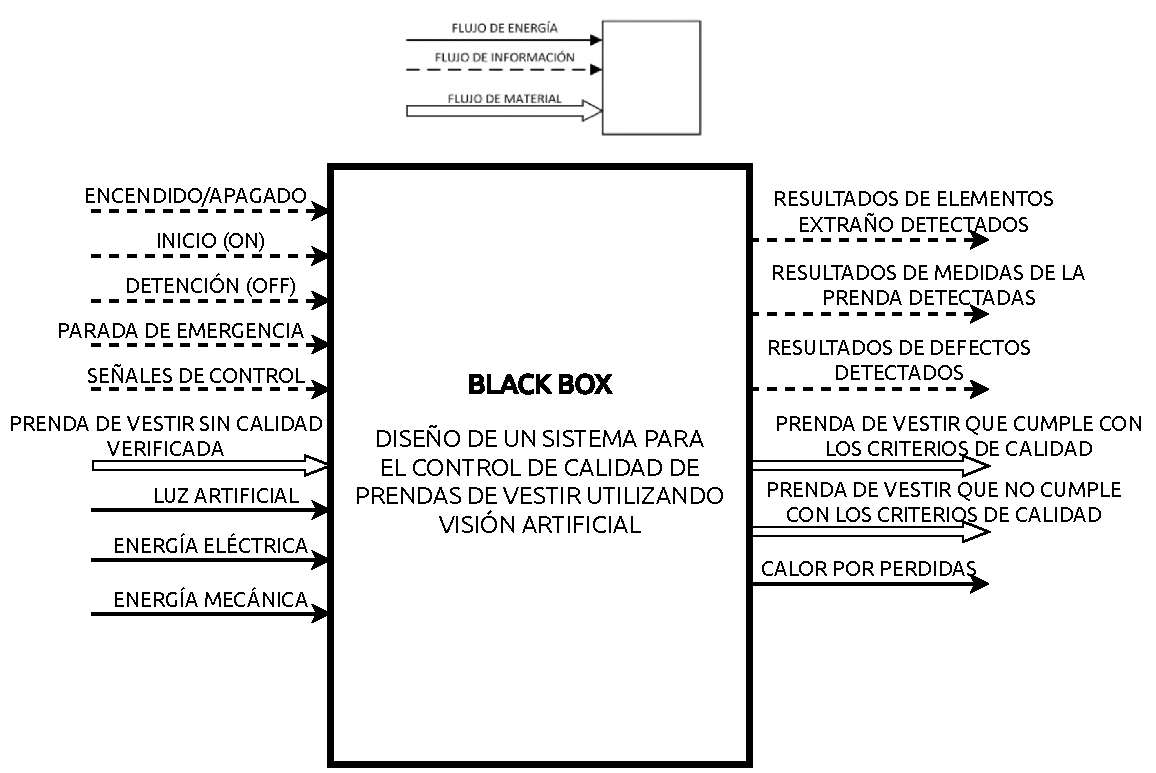
\includegraphics[width=\textwidth]{img/BLACK_BOX.drawio.pdf}
    \caption[Black Box.]{Black Box. Fuente: Elaboración propia.}
    \label{fig:BLACK_BOX}
\end{figure}

\subsection{Funciones Parciales}
\label{Funciones Parciales}

Aquellos procesos que interactúan directamente con el material a ser analizado conforman las funciones básicas del sistema. Estas funciones se muestran en la Figura \ref{fig:ESTRUCTURA_DE_FUNCIONES}. Primero, prendas de vestir sin clasificar son ingresadas por un operario para iniciar el proceso de detección de defectos. Se debe contar además con algún método que maximice la superficie de la prenda que pueda ser visible para la cámara, con el fin de incrementar la efectividad del proceso de detección y clasificación según los criterios de selección. Luego esta prenda es analizada mediante módulos especializados en la detección de defectos visuales y otro módulo encargado de identificar la presencia de elementos metálicos extraños. Como resultado de este proceso, se producirá una imagen que resalta los defectos detectados en la prenda donde se señala la existencia o no de elementos metálicos ajenos. Finalmente, las prendas ya verificadas serán transportadas a la disposición final adecuada.

\begin{sidewaysfigure}
	\begin{figure}[H]
		\centering
		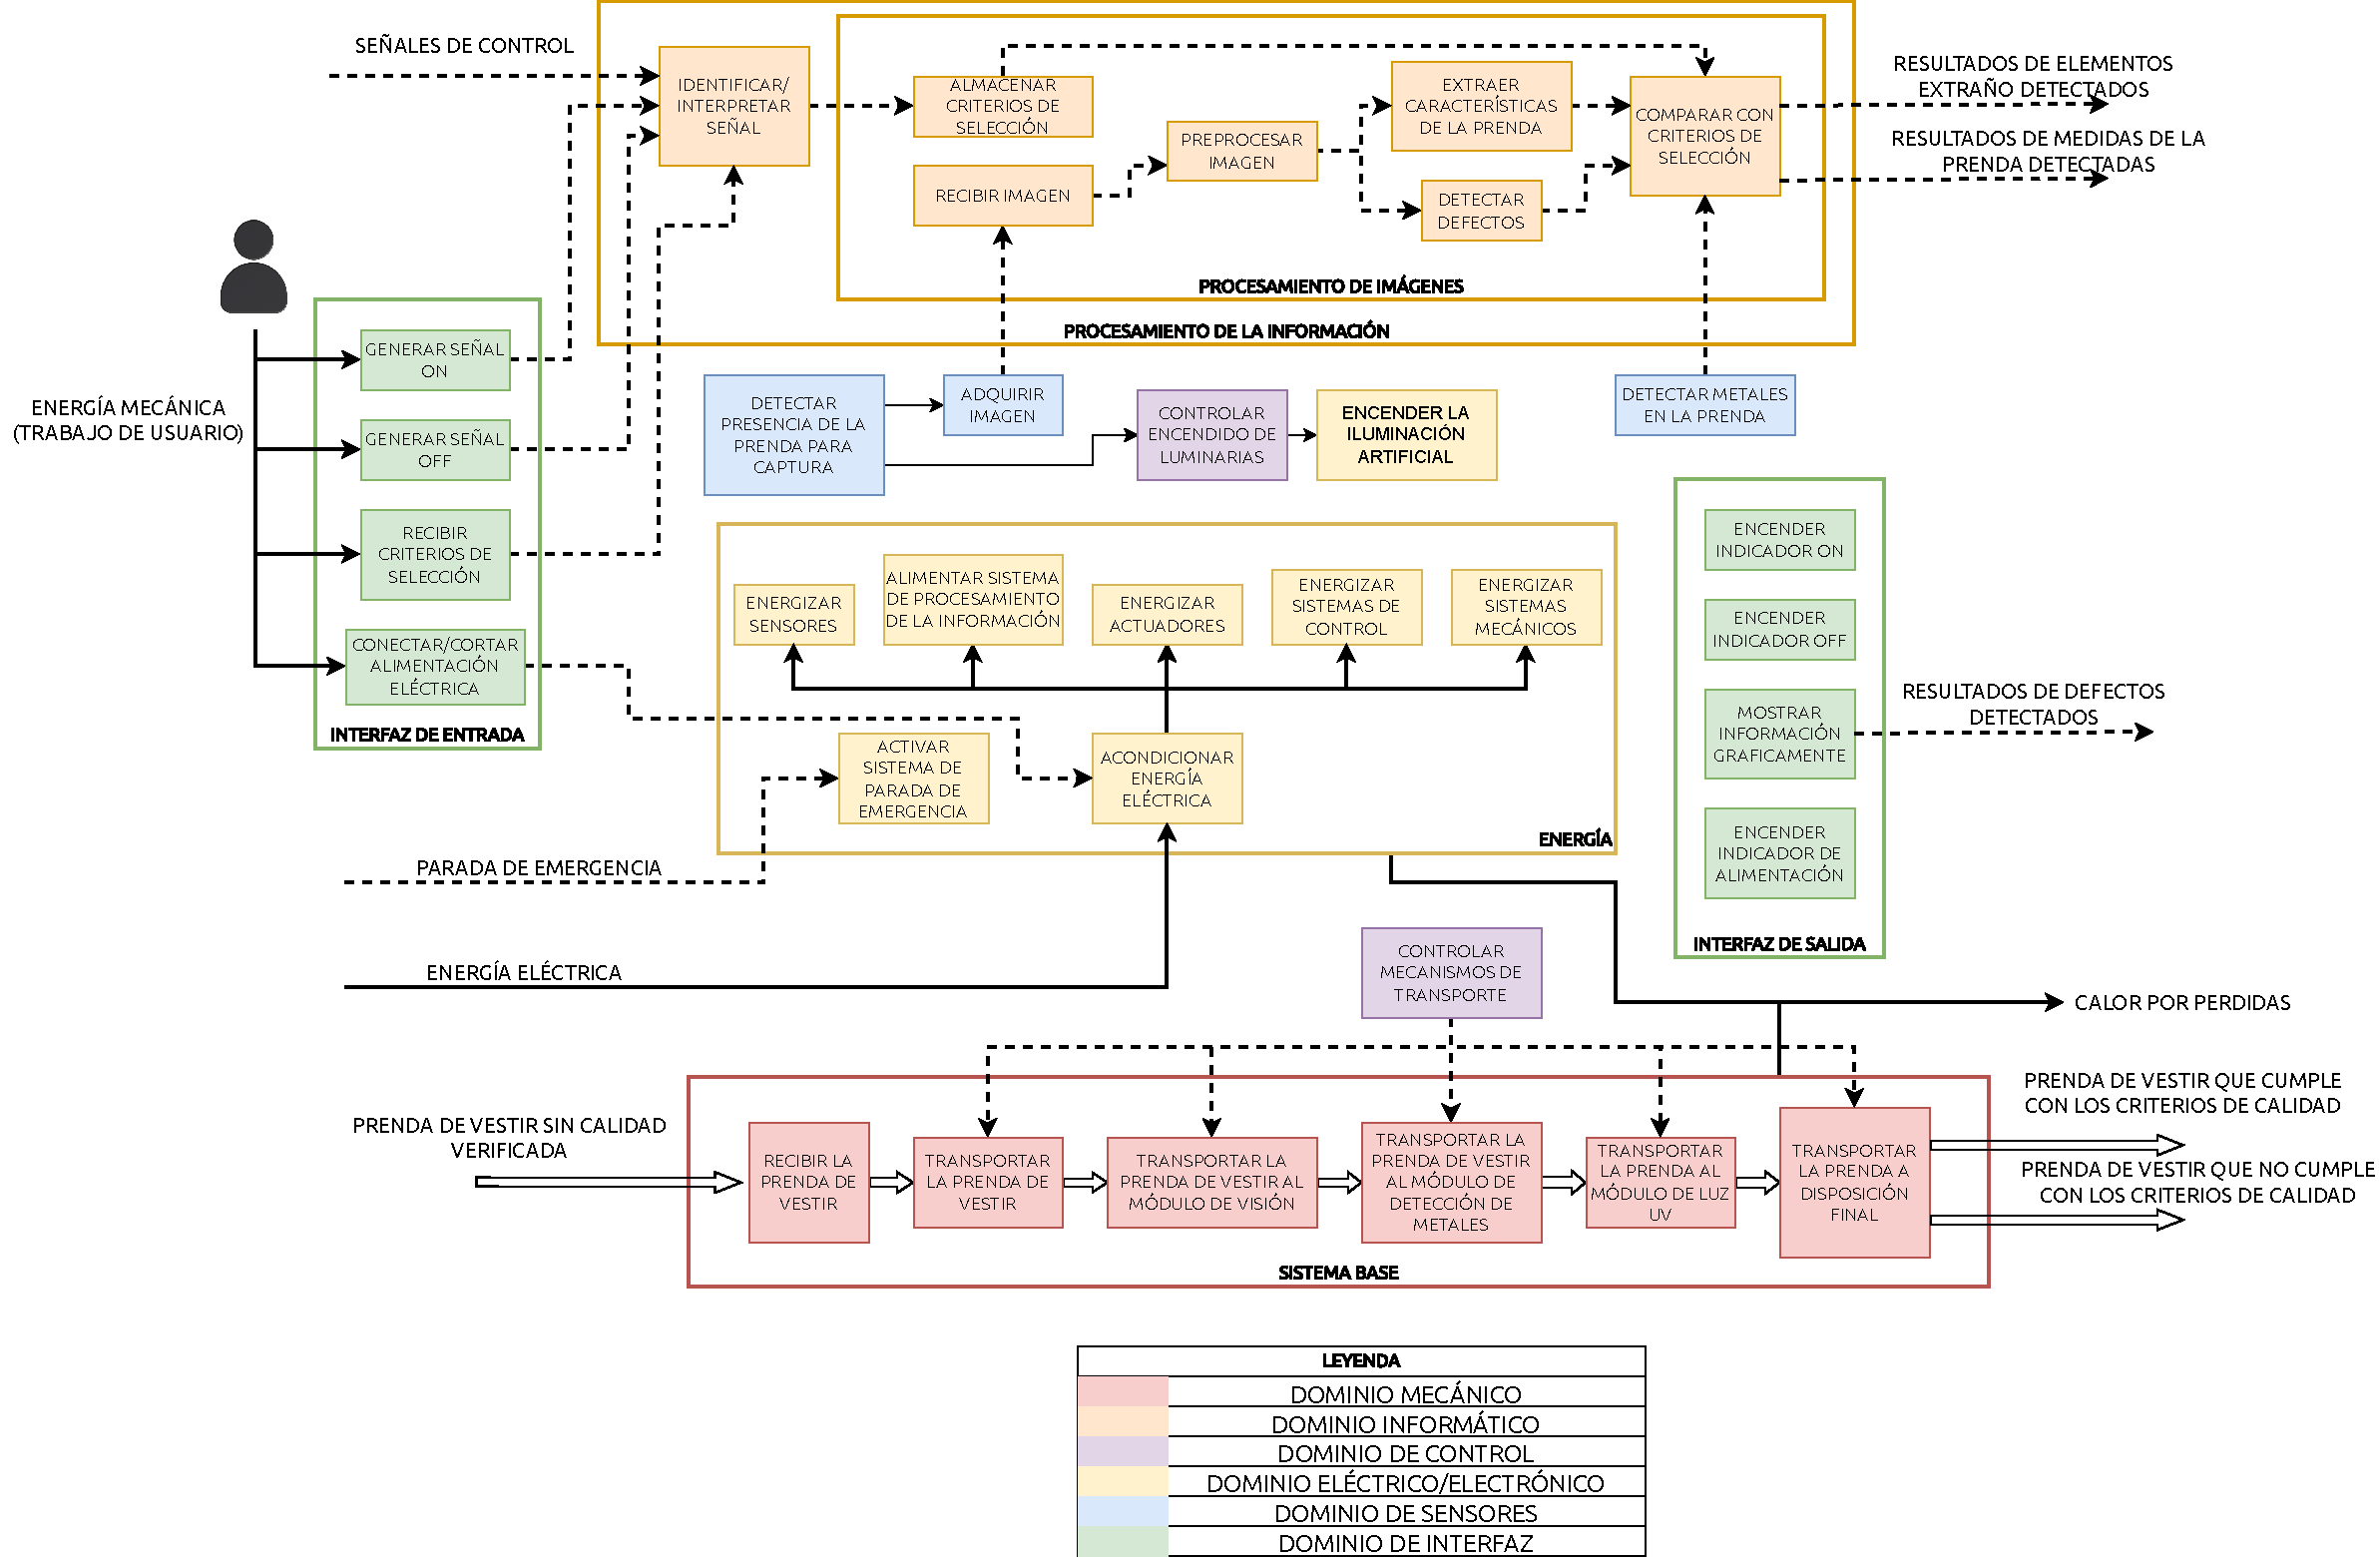
\includegraphics[width=\textwidth]{img/ESTRUCTURA_DE_FUNCIONES.drawio.pdf}
		\label{fig:ESTRUCTURA_DE_FUNCIONES}
		\caption[Estructura de funciones del sistema.]{Estructura de funciones del sistema. Fuente: Elaboración propia.}
	\end{figure}
\end{sidewaysfigure}

\subsubsection{Dominio Mecánico}

El dominio mecánico abarca todas las operaciones físicas y movimientos asociados con el manejo de prendas de vestir, como se muestra en la Figura \ref{fig:EF_DM}. Incluye la recepción de las prendas, su transporte a través de diferentes estaciones de procesamiento como módulos de visión artificial y detección de metales. Este dominio garantiza que las prendas se muevan eficientemente de una etapa a otra, facilitando su análisis y clasificación según cumplan o no con los criterios de calidad establecidos.

\begin{figure}[h]
	\centering
	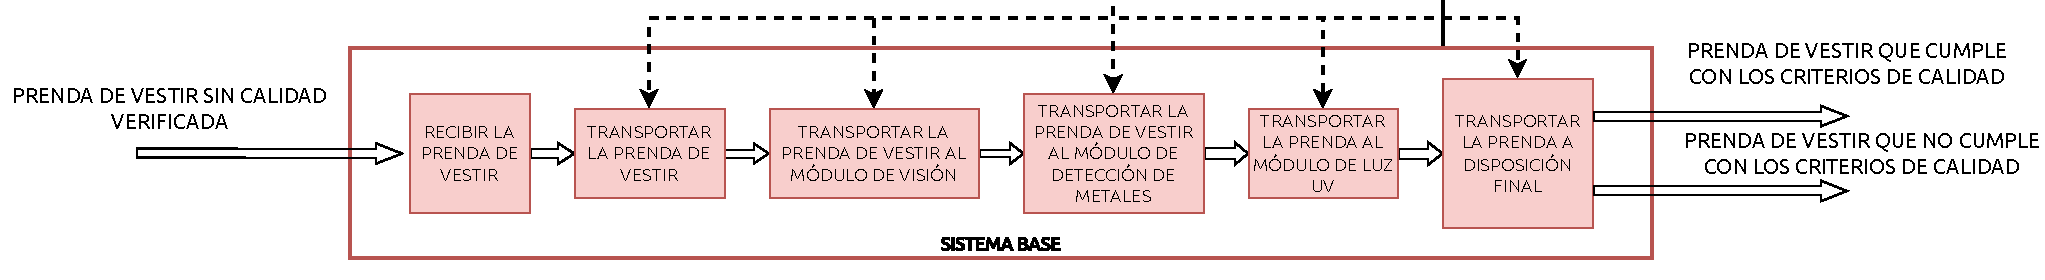
\includegraphics[width=\textwidth]{img/EF_DM.pdf}
	\caption[Estructura de funciones del dominio mecánico.]{Estructura de funciones del dominio mecánico. Fuente: Elaboración propia.}
	\label{fig:EF_DM}
\end{figure}

\subsubsection{Dominio Informático}

El dominio informático se centra en el procesamiento de la información obtenida de las prendas , como se muestra en la Figura \ref{fig:EF_DIn}. Este dominio comprende la adquisición y preprocesamiento de imágenes de las prendas, extracción de características relevantes, detección de defectos, y comparación de estos datos con criterios de selección predefinidos para determinar la calidad de las prendas. Este dominio es crucial para interpretar los datos capturados y tomar decisiones basadas en la información procesada.

\begin{figure}[h]
	\centering
	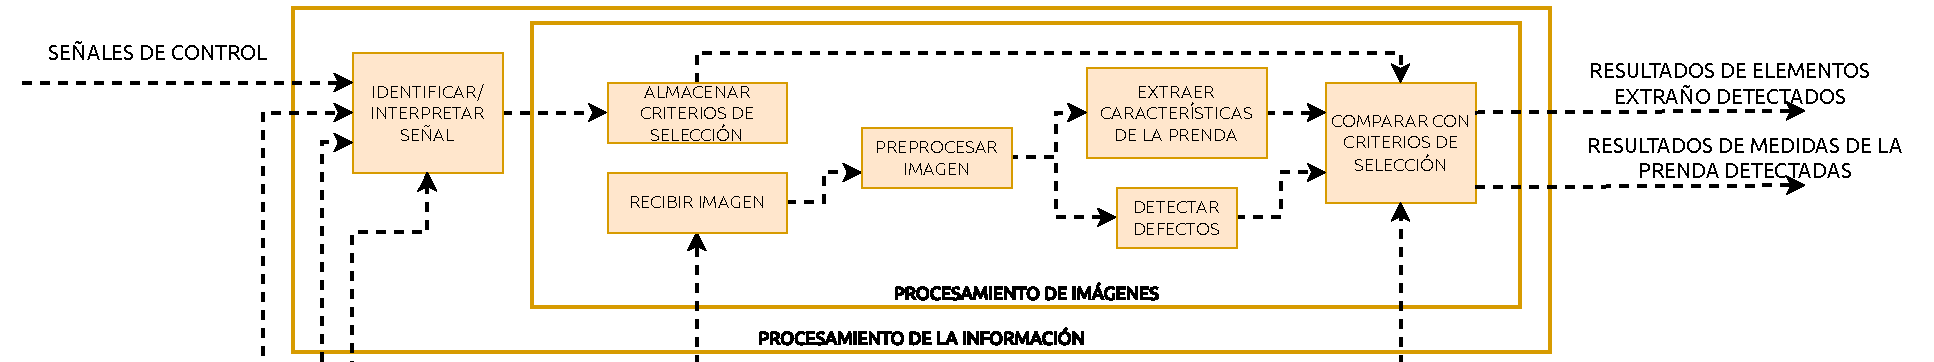
\includegraphics[width=\textwidth]{img/EF_DIn.pdf}
	\caption[Estructura de funciones del dominio informático.]{Estructura de funciones del dominio informático. Fuente: Elaboración propia.}
	\label{fig:EF_DIn}
\end{figure}

\subsubsection{Dominio de Control}

El dominio de control, mostrado en la Figura \ref{fig:EF_DC}, incluye la lógica de control y los mecanismos de decisión que guían las operaciones del sistema. Esto implica generar señales de encendido/apagado basadas en la información procesada, manejar interfaces de entrada/salida, y activar mecanismos de parada de emergencia. Este dominio es esencial para coordinar las actividades de los otros dominios y asegurar que el sistema responda adecuadamente a las condiciones de operación y a los requisitos de procesamiento.

\begin{figure}[h]
	\centering
	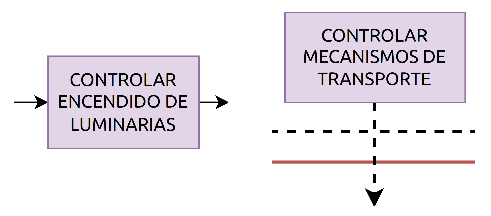
\includegraphics[width=0.4\textwidth]{img/EF_DC.pdf}
	\caption[Estructura de funciones del dominio de control.]{Estructura de funciones del dominio de control. Fuente: Elaboración propia.}
	\label{fig:EF_DC}
\end{figure}

\subsubsection{Dominio Eléctrico/Electrónico}

Este dominio se ocupa de la alimentación y control eléctrico de todos los componentes del sistema, tal y como se muestra en la Figura \ref{fig:EF_DEE}. Desde energizar los sensores hasta alimentar los sistemas de procesamiento de información, actuadores, y sistemas de control, este dominio asegura que todos los elementos electrónicos del sistema reciban la energía necesaria para su funcionamiento. Además, gestiona la iluminación necesaria para la adquisición de imágenes y la señalización a través de indicadores ON/OFF.

\begin{figure}[h]
	\centering
	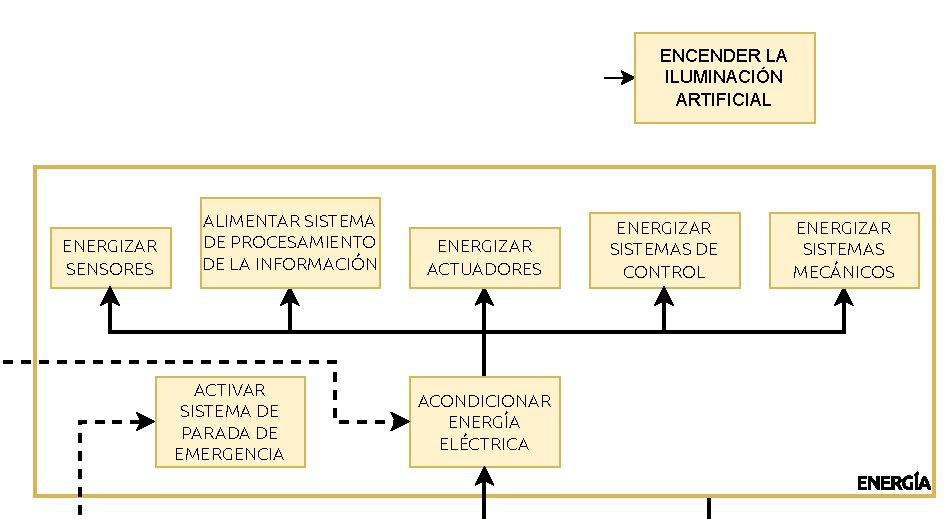
\includegraphics[width=0.8\textwidth]{img/EF_DEE.pdf}
	\caption[Estructura de funciones del dominio eléctrico/electrónico.]{Estructura de funciones del dominio eléctrico/electrónico. Fuente: Elaboración propia.}
	\label{fig:EF_DEE}
\end{figure}

\subsubsection{Dominio de Sensores}

Este dominio comprende la detección y recopilación de datos a través de sensores diseñados para identificar características específicas de las prendas. Esto se muestra en la Figura \ref{fig:EF_DS}. Se identifica la presencia de metales o la preparación para la captura de imágenes. La información recogida por los sensores es vital para el adecuado funcionamiento del sistema, ya que permite adaptar las operaciones a las condiciones actuales y a las necesidades específicas de procesamiento de las prendas.

\begin{figure}[h]
	\centering
	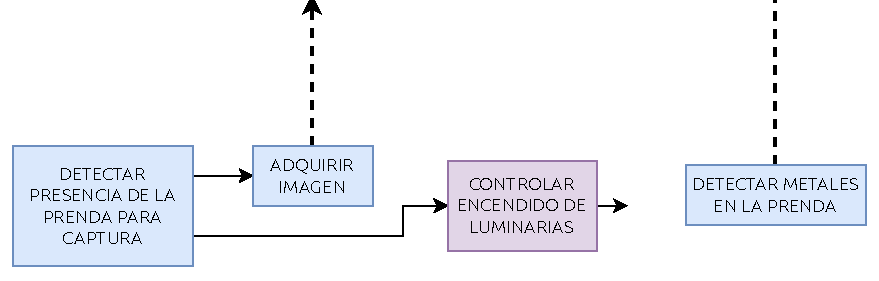
\includegraphics[width=0.7\textwidth]{img/EF_DS.pdf}
	\caption[Estructura de funciones del dominio de sensores.]{Estructura de funciones del dominio de sensores. Fuente: Elaboración propia.}
	\label{fig:EF_DS}
\end{figure}

\subsubsection{Dominio de Interfaz}

El dominio de interfaz esta dedica en interactuar con los usuarios finales del sistema. Como se muestra en la Figura \ref{fig:EF_DI}, a través del empleo de la energía mecánica del operario del sistema para generar las señales de control, lo cual incluye la señal de encendido, apagado o de parada de emergencia. Por otro lado, La información de los resultados de todos los procesos realizados por el sistema se mostraran mediante una interfaz que las muestre de manera ordenada y concisa.

\begin{figure}[h]
	\centering
	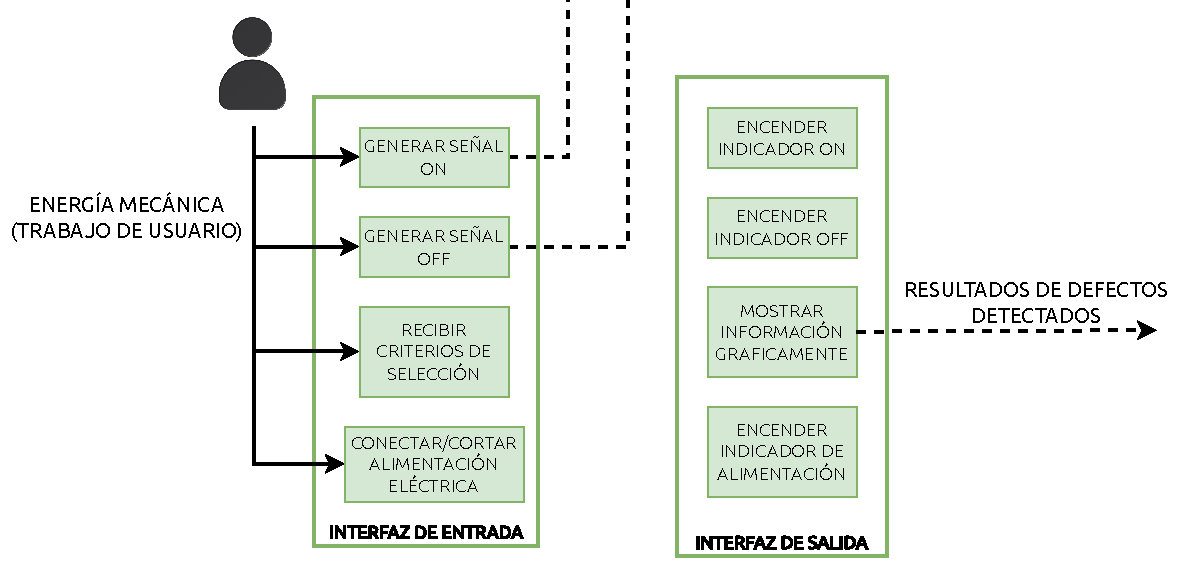
\includegraphics[width=\textwidth]{img/EF_DI.pdf}
	\caption[Estructura de funciones del dominio de interfaz.]{Estructura de funciones del dominio de interfaz. Fuente: Elaboración propia.}
	\label{fig:EF_DI}
\end{figure}

\section{Matriz morfológica}

A continuación, se presentan las diferentes matrices morfológicas para cada dominio previamente descrito, esta metodología ayudó a visualizar las diferentes opciones y escoger una solución idónea para los requerimientos. En las Tablas \ref{tab:MM_DI}, \ref{tab:MM_DM}, \ref{tab:MM_DIn}, \ref{tab:MM_DC}, \ref{tab:MM_DEE} y \ref{tab:MM_DS} se observan las matrices morfológicas del dominio de interfaz, dominio mecánico, dominio informático, dominio de control, dominio eléctrico/electrónico y dominio de sensores respectivamente. 
Las cuatro alternativas de solución se clasificarán siguiendo la leyenda de colores mostrada en la Tabla \ref{tab:leyenda_colores_soluciones}. Estos soluciones se generan al colocar un $\B{\blacklozenge}{1.35}$ con el color correspondiente al concepto de solución para cada función parcial de las matrices morfológicas.

\begin{table}[H]
	\centering
	\caption[Leyenda de colores para los conceptos de solución en las matriz morfológica.]{Leyenda de colores para los conceptos de solución en las matriz morfológica. Fuente: Elaboración propia.}
	\begin{tabular}{|c|c|c|}
		\hline
		\textbf{Soluciones} & \textbf{Tipo de Solución} & \textbf{Color} \bigstrut\\
		\hline
		Solución 1 & Accesible & \cellcolor[rgb]{ 1,  0,  0} \bigstrut\\
		\hline
		Solución 2 & Robusta & \cellcolor[rgb]{ 0,  0,  1} \bigstrut\\
		\hline
		Solución 3 & Precisa & \cellcolor[rgb]{ .298,  .835,  .078} \bigstrut\\
		\hline
	\end{tabular}%
	\label{tab:leyenda_colores_soluciones}%
\end{table}

% ==================== LEYENDA PARA 4 CONCEPTOS DE SOLUCIÓN ====================
%\begin{table}[H]
%	\centering
%	\caption[Leyenda de colores de los conceptos de solución generados en las matrices
%	morfológicas.]{Leyenda de colores de los conceptos de solución generados en las matrices
%		morfológicas. Fuente: Elaboración propia.}
%	\begin{tabular}{|c|c|c|}
%		\hline
%		\textbf{Soluciones} & \textbf{Tipo de Solución} & \textbf{Color} \bigstrut\\
%		\hline
%		Solución 1 & Económica & \cellcolor[rgb]{ 1,  0,  0} \bigstrut\\
%		\hline
%		Solución 2 & Robusta & \cellcolor[rgb]{ 0,  0,  1} \bigstrut\\
%		\hline
%		Solución 3 & Equilibrada & \cellcolor[rgb]{ .298,  .835,  .078} \bigstrut\\
%		\hline
%		Solución 4 & Rápida & \cellcolor[rgb]{ 1,  .502,  0} \bigstrut\\
%		\hline
%	\end{tabular}%
%	\label{tab:leyenda_colores_soluciones}%
%\end{table}


% ==================== PLANTILLA PARA DOMINIO CON 3 SOLUCIONES ====================
%\begin{longtable}{|M{\anchoFPT}|C{6em}|C{6em}|C{6em}|}
%	\caption{Matriz morfológica del dominio de interfaz.}\label{tab:MM_DI}\\
%	\hline
%	\multirow{2}{\anchoFPT}{\parbox{\anchoFPT}{\centering \textbf{FUNCIONES PARCIALES}}} & \multicolumn{3}{c|}{\textbf{DOMINIO INTERFAZ}} \bigstrut\\
%	\cline{2-4} & \textbf{OPCIÓN 1} & \textbf{OPCIÓN 2} & \textbf{OPCIÓN 3} \bigstrut\\
%	\hline
%	\endfirsthead
%	\caption* {Tabla \ref{tab:MM_DI}: Matriz morfológica del dominio de interfaz (Continuación).}\\
%	\hline
%	\multirow{2}{\anchoFPT}{\parbox{\anchoFPT}{\centering \textbf{FUNCIONES PARCIALES}}} & \multicolumn{3}{c|}{\textbf{DOMINIO INTERFAZ}} \bigstrut\\
%	\cline{2-4} & \textbf{OPCIÓN 1} & \textbf{OPCIÓN 2} & \textbf{OPCIÓN 3} \bigstrut\\
%	\hline
%	\endhead
%	\multirow{2}{\anchoFPT}{GENERAR SEÑAL ON Y GENERAR SEÑAL OFF} & \IMM{0.08}{img/botonera1.jpg}{1em} & \IMM{0.1}{img/boton_enc_apa_GUI.jpg}{0.6em} & \IMM{0.12}{img/Switch_tipo_perilla.jpeg}{0.3em} \bigstrut\\
%	\cline{2-4} & Caja con pulsador Start-Stop. \OpR & Botones ON/OFF en GUI. \OpV & Interruptor tipo perilla. \OpA \bigstrut\\
%	\hline
%	\multirow{2}{\anchoFPT}{ENCENDER INDICADOR ON Y ENCENDER INDICADOR OFF} & \IMM{0.13}{img/pilotos_led.jpg}{0.5em} & \IMM{0.14}{img/pantalla_LCD.jpg}{0.3em} & \IMM{0.15}{img/GUI.jpg}{0.1em} \bigstrut\\
%	\cline{2-4} & Pilotos led. \OpA & Pantalla LCD. \OpR & GUI. \OpV \bigstrut\\
%	\hline
%	\multirow{2}{\anchoFPT}{RECIBIR CRITERIOS DE SELECCIÓN} & \IMM{0.13}{img/hmi_industrial.png}{0.2em} & \IMM{0.15}{img/Pantalla_Perilla.jpg}{0.24em} & \IMM{0.15}{img/GUI.jpg}{0.1em} \bigstrut\\
%	\cline{2-4} & HMI Indsutrial. \OpA & Pantalla LCD con perilla de control \OpN & GUI. \OpV \bigstrut\\
%	\hline
%	\multirow{2}{\anchoFPT}{CONECTAR Y CORTAR ALIMENTACIÓN ELÉCTRICA} & \IMM{0.12}{img/termomagnético_diferencial.jpg}{0.7em} & \IMM{0.11}{img/Conmutador_industrial.jpeg}{0.2em} & \IMM{0.11}{img/cable_interruptor.jpg}{0.1em} \bigstrut\\
%	\cline{2-4} & Diferencial con Termomagnético. \OpA \OpV & Conmutador Industrial. \OpN & Cable, enchufe e interruptor. \OpR \bigstrut\\
%	\hline
%	\multirow{2}{\anchoFPT}{MOSTRAR INFORMACIÓN GRAFICAMENTE} & \IMM{0.13}{img/hmi_industrial.png}{0.2em} & \IMM{0.15}{img/GUI.jpg}{0.1em} & \bigstrut\\
%	\cline{2-4} & HMI Indsutrial. \OpR \OpV & GUI.\OpA \OpN &  \bigstrut\\
%	\hline
%\end{longtable}

% =======================================================
%\begin{longtable}{|M{\anchoFPT}|C{6em}|C{6em}|C{6em}|}
%	\caption{Matriz morfológica del dominio de interfaz.}\label{tab:MM_DI}\\
%	\hline
%	\multirow{2}{\anchoFPT}{\parbox{\anchoFPT}{\centering \textbf{FUNCIONES PARCIALES}}} & \multicolumn{3}{c|}{\textbf{DOMINIO }} \bigstrut\\
%	\cline{2-4} & \textbf{OPCIÓN 1} & \textbf{OPCIÓN 2} & \textbf{OPCIÓN 3} \bigstrut\\
%	\hline
%	\endfirsthead
%	\caption* {Tabla \ref{tab:MM_DI}: Matriz morfológica del dominio de interfaz (Continuación).}\\
%	\hline
%	\multirow{2}{\anchoFPT}{\parbox{\anchoFPT}{\centering \textbf{FUNCIONES PARCIALES}}} & \multicolumn{3}{c|}{\textbf{DOMINIO }} \bigstrut\\
%	\cline{2-4} & \textbf{OPCIÓN 1} & \textbf{OPCIÓN 2} & \textbf{OPCIÓN 3} \bigstrut\\
%	\hline
%	\endhead
%	\multirow{2}{\anchoFPT}{} & \IMM{0.08}{img/botonera1.jpg}{1em} & \IMM{0.1}{img/boton_enc_apa_GUI.jpg}{0.6em} & \IMM{0.12}{img/Switch_tipo_perilla.jpeg}{0.3em} \bigstrut\\
%	\cline{2-4} & Caja con pulsador Start-Stop. \OpR & Botones ON/OFF en GUI. \OpV & Interruptor tipo perilla. \OpA \bigstrut\\
%	\hline
%\end{longtable}

\subsection{Dominio de Interfaz}

\begin{longtable}{|M{\anchoFPT}|C{6em}|C{6em}|C{6em}|}
	\caption{Matriz morfológica del dominio de interfaz.}\label{tab:MM_DI}\\
	\hline
	\multirow{2}{\anchoFPT}{\parbox{\anchoFPT}{\centering \textbf{FUNCIONES PARCIALES}}} & \multicolumn{3}{c|}{\textbf{DOMINIO INTERFAZ}} \bigstrut\\
	\cline{2-4} & \textbf{OPCIÓN 1} & \textbf{OPCIÓN 2} & \textbf{OPCIÓN 3} \bigstrut\\
	\hline
	\endfirsthead
	\caption* {Tabla \ref{tab:MM_DI}: Matriz morfológica del dominio de interfaz (Continuación).}\\
	\hline
	\multirow{2}{\anchoFPT}{\parbox{\anchoFPT}{\centering \textbf{FUNCIONES PARCIALES}}} & \multicolumn{3}{c|}{\textbf{DOMINIO INTERFAZ}} \bigstrut\\
	\cline{2-4} & \textbf{OPCIÓN 1} & \textbf{OPCIÓN 2} & \textbf{OPCIÓN 3} \bigstrut\\
	\hline
	\endhead
	\multirow{2}{\anchoFPT}{GENERAR SEÑAL ON Y GENERAR SEÑAL OFF} & \IMM{0.08}{img/botonera1.jpg}{1em} & \IMM{0.1}{img/boton_enc_apa_GUI.jpg}{0.6em} & \IMM{0.12}{img/Switch_tipo_perilla.jpeg}{0.3em} \bigstrut\\
	\cline{2-4} & Caja con pulsador Start-Stop. \OpV & Botones ON/OFF en GUI. \OpR & Interruptor tipo perilla. \OpA \bigstrut\\
	\hline
	\multirow{2}{\anchoFPT}{ENCENDER INDICADOR ON Y ENCENDER INDICADOR OFF} & \IMM{0.13}{img/pilotos_led.jpg}{0.5em} & \IMM{0.14}{img/pantalla_LCD.jpg}{0.3em} & \IMM{0.15}{img/GUI.jpg}{0.1em} \bigstrut\\
	\cline{2-4} & Pilotos led. \OpA & Pantalla LCD. \OpR & GUI. \OpV \bigstrut\\
	\hline
	\multirow{2}{\anchoFPT}{RECIBIR CRITERIOS DE SELECCIÓN} & \IMM{0.13}{img/hmi_industrial.png}{0.2em} & \IMM{0.15}{img/Pantalla_Perilla.jpg}{0.24em} & \IMM{0.15}{img/GUI.jpg}{0.1em} \bigstrut\\
	\cline{2-4} & HMI Indsutrial. \OpA & Pantalla LCD con perilla de control \OpR & GUI. \OpV \bigstrut\\
	\hline
	\multirow{2}{\anchoFPT}{CONECTAR Y CORTAR ALIMENTACIÓN ELÉCTRICA} & \IMM{0.12}{img/termomagnético_diferencial.jpg}{0.7em} & \IMM{0.11}{img/Conmutador_industrial.jpeg}{0.2em} & \IMM{0.11}{img/cable_interruptor.jpg}{0.1em} \bigstrut\\
	\cline{2-4} & Diferencial con Termomagnético. \OpA & Conmutador Industrial. \OpV & Cable, enchufe e interruptor. \OpR \bigstrut\\
	\hline
	\multirow{2}{\anchoFPT}{MOSTRAR INFORMACIÓN GRAFICAMENTE} & \IMM{0.13}{img/hmi_industrial.png}{0.2em} & \IMM{0.15}{img/GUI.jpg}{0.1em} & \bigstrut\\
	\cline{2-4} & HMI Indsutrial. \OpA & GUI.\OpR \OpV &  \bigstrut\\
	\hline
\end{longtable}

%\begin{longtable}{|p{\anchoFP}|C{6em}|C{6em}|C{6em}|C{6em}|}
%	\caption{Matriz morfológica del dominio de interfaz.}\label{tab:MM_DIA}\\
%	\hline
%	\multirow{2}{\anchoFP}{\textbf{FUNCIONES PARCIALES}} & \multicolumn{4}{C{24em}|}{\textbf{DOMINIO DE INTERFAZ}} \bigstrut\\
%	\cline{2-5} & \multicolumn{1}{C{6em}|}{\textbf{OPCIÓN 1}} & \multicolumn{1}{C{6em}|}{\textbf{OPCIÓN 2}} & \multicolumn{1}{C{6em}|}{\textbf{OPCIÓN 3}} & \multicolumn{1}{C{6em}|}{\textbf{OPCIÓN 4}} \bigstrut\\
%	\hline
%	\endfirsthead
%	\caption* {Tabla \ref{tab:MM_DI}: Matriz morfológica del dominio de interfaz (Continuación).}\\
%	\hline
%	\multirow{2}{\anchoFP}{\textbf{FUNCIONES PARCIALES}} & \multicolumn{4}{C{24em}|}{\textbf{DOMINIO DE INTERFAZ}} \bigstrut\\
%	\cline{2-5} & \multicolumn{1}{C{6em}|}{\textbf{OPCIÓN 1}} & \multicolumn{1}{C{6em}|}{\textbf{OPCIÓN 2}} & \multicolumn{1}{C{6em}|}{\textbf{OPCIÓN 3}} & \multicolumn{1}{C{6em}|}{\textbf{OPCIÓN 4}} \bigstrut\\
%	\hline
%	\endhead
%	\multirow{2}{\anchoFP}{GENERAR SEÑAL ON Y GENERAR SEÑAL OFF} & \IMM{0.08}{img/botonera1.jpg}{1em} & \IMM{0.1}{img/boton_enc_apa_GUI.jpg}{0.6em}& \IMM{0.12}{img/Switch_tipo_perilla.jpeg}{0.3em} &\IMM{0.13}{img/Interruptor_tipo_palanca.jpg}{0.3em} \bigstrut\\
%	\cline{2-5} & Caja con pulsador Start-Stop. \OpN & Botones ON/OFF en GUI. \OpV & Interruptor tipo perilla. \OpA & Switch de palanca. \OpR \bigstrut\\
%	\hline	
%	\multirow{2}{\anchoFP}{ENCENDER INDICADOR ON Y ENCENDER INDICADOR OFF} & \IMM{0.12}{img/leds.jpg}{0.7em} & \IMM{0.13}{img/pilotos_led.jpg}{0.5em}& \IMM{0.14}{img/pantalla_LCD.jpg}{0.3em} &\IMM{0.15}{img/GUI.jpg}{0.1em} \bigstrut\\
%	\cline{2-5} & Luces LED. \OpR & Pilotos led. \OpA & Pantalla LCD. \OpN & GUI. \OpV \bigstrut\\
%	\hline
%	\multirow{2}{\anchoFP}{RECIBIR CRITERIOS DE SELECCIÓN} & \IMM{0.13}{img/hmi_industrial.png}{0.2em} & \IMM{0.12}{img/pantalla_tactil.jpg}{0.05em}& \IMM{0.15}{img/Pantalla_Perilla.jpg}{0.24em} & \IMM{0.15}{img/GUI.jpg}{0.1em} \bigstrut\\
%	\cline{2-5} & HMI Indsutrial. \OpA & Pantalla Táctil. \OpR & Pantalla LCD con perilla de control \OpN & GUI. \OpV \bigstrut\\
%	\hline
%	\multirow{2}{\anchoFP}{CONECTAR Y CORTAR ALIMENTACIÓN ELÉCTRICA} & \IMM{0.12}{img/termomagnético_diferencial.jpg}{0.7em} & \IMM{0.11}{img/Conmutador_industrial.jpeg}{0.2em} & \IMM{0.11}{img/cable_interruptor.jpg}{0.1em} & \bigstrut\\
%	\cline{2-5} & Diferencial con Termomagnético. \OpA \OpV & Conmutador Industrial. \OpN & Cable, enchufe e interruptor. \OpR & \bigstrut\\
%	\hline
%	\multirow{2}{\anchoFP}{MOSTRAR INFORMACIÓN GRAFICAMENTE} & \IMM{0.14}{img/hmi_industrial.png}{0.1em} & \IMM{0.15}{img/GUI.jpg}{0.1em} &  &  \bigstrut\\
%	\cline{2-5} & HMI Indsutrial. \OpR \OpV & GUI.\OpA \OpN & & \bigstrut\\
%	\hline
%\end{longtable}

\subsection{Dominio Mecánico}

\begin{longtable}{|M{\anchoFPT}|C{6em}|C{6em}|C{6em}|}
	\caption{Matriz morfológica del dominio mecánico.}\label{tab:MM_DM}\\
	\hline
	\multirow{2}{\anchoFPT}{\parbox{\anchoFPT}{\centering \textbf{FUNCIONES PARCIALES}}} & \multicolumn{3}{c|}{\textbf{DOMINIO MECÁNICO}} \bigstrut\\
	\cline{2-4} & \textbf{OPCIÓN 1} & \textbf{OPCIÓN 2} & \textbf{OPCIÓN 3} \bigstrut\\
	\hline
	\endfirsthead
	\caption* {Tabla \ref{tab:MM_DM}: Matriz morfológica del dominio mecánico (Continuación).}\\
	\hline
	\multirow{2}{\anchoFPT}{\parbox{\anchoFPT}{\centering \textbf{FUNCIONES PARCIALES}}} & \multicolumn{3}{c|}{\textbf{DOMINIO MECÁNICO}} \bigstrut\\
	\cline{2-4} & \textbf{OPCIÓN 1} & \textbf{OPCIÓN 2} & \textbf{OPCIÓN 3} \bigstrut\\
	\hline
	\endhead
	\multirow{2}{\anchoFPT}{TRANSPORTE MECÁNICO DE LAS PRENDAS DE VESTIR} & \IMM{0.14}{img/faja_transportadora_plana.jpg}{0.2em} & \IMM{0.13}{img/faja_transportadora_inclinada.jpg}{0.8em}& \IMM{0.11}{img/conveyer.jpg}{0.2em} \bigstrut\\
	\cline{2-4} & Faja transportadora plana. & Faja transportadora inclinada. & Transportador automático de ropa. \bigstrut\\
	\hline	
	\multirow{2}{\anchoFPT}{GENERAR EL MOVIMIENTO DEL SISTEMA DE TRANSPORTE} & \IMM{0.15}{img/stepper_motor.jpg}{0.3em} & \IMM{0.15}{img/motor_sincrono.jpg}{0.1em}& \IMM{0.14}{img/motor_asincrono.jpg}{0.2em} \bigstrut\\
	\cline{2-4} & Motor a pasos. \OpV & Motor síncrono. \OpA & Motor de inducción. \OpR \bigstrut\\
	\hline
\end{longtable}

%\begin{longtable}{|p{\anchoFP}|C{6em}|C{6em}|C{6em}|C{6em}|}
%	\caption{Matriz morfológica del dominio mecánico.}\label{tab:MM_DM}\\
%	\hline
%	\multirow{2}{\anchoFP}{\textbf{FUNCIONES PARCIALES}} & \multicolumn{4}{C{24em}|}{\textbf{DOMINIO MECÁNICO}} \bigstrut\\
%	\cline{2-5} & \multicolumn{1}{C{6em}|}{\textbf{OPCIÓN 1}} & \multicolumn{1}{C{6em}|}{\textbf{OPCIÓN 2}} & \multicolumn{1}{C{6em}|}{\textbf{OPCIÓN 3}} & \multicolumn{1}{C{6em}|}{\textbf{OPCIÓN 4}} \bigstrut\\
%	\hline
%	\endfirsthead
%	\caption* {Tabla \ref{tab:MM_DM}: Matriz morfológica del dominio mecánico. (Continuación).}\\
%	\hline
%	\multirow{2}{\anchoFP}{\textbf{FUNCIONES PARCIALES}} & \multicolumn{4}{C{24em}|}{\textbf{DOMINIO MECÁNICO}} \bigstrut\\
%	\cline{2-5} & \multicolumn{1}{C{6em}|}{\textbf{OPCIÓN 1}} & \multicolumn{1}{C{6em}|}{\textbf{OPCIÓN 2}} & \multicolumn{1}{C{6em}|}{\textbf{OPCIÓN 3}} & \multicolumn{1}{C{6em}|}{\textbf{OPCIÓN 4}} \bigstrut\\
%	\hline
%	\endhead
%	\multirow{2}{\anchoFP}{TRANSPORTE MECÁNICO DE LAS PRENDAS DE VESTIR} & \IMM{0.14}{img/faja_transportadora_plana.jpg}{0.2em} & \IMM{0.13}{img/faja_transportadora_inclinada.jpg}{0.8em}& \IMM{0.11}{img/conveyer.jpg}{0.2em} &\bigstrut\\
%	\cline{2-5} & Faja transportadora plana. \OpA & Faja transportadora inclinada. \OpR & Transportador automático de ropa. \OpV \OpN& \bigstrut\\
%	\hline	
%	\multirow{2}{\anchoFP}{GENERAR EL MOVIMIENTO DEL SISTEMA DE TRANSPORTE} & \IMM{0.15}{img/stepper_motor.jpg}{0.3em} & \IMM{0.15}{img/motor_sincrono.jpg}{0.1em}& \IMM{0.14}{img/motor_asincrono.jpg}{0.2em} &\IMM{0.14}{img/BLDC.jpg}{0.2em} \bigstrut\\
%	\cline{2-5} & Motor a pasos. \OpA & Motor síncrono. \OpN & Motor de inducción. \OpV & Motor BLDC. \OpR \bigstrut\\
%	\hline
%\end{longtable}

\subsection{Dominio Informático}

\begin{longtable}{|M{\anchoFPT}|C{6em}|C{6em}|C{6em}|}
	\caption{Matriz morfológica del dominio informático.}\label{tab:MM_DIn}\\
	\hline
	\multirow{2}{\anchoFPT}{\parbox{\anchoFPT}{\centering \textbf{FUNCIONES PARCIALES}}} & \multicolumn{3}{c|}{\textbf{DOMINIO INFORMÁTICO}} \bigstrut\\
	\cline{2-4} & \textbf{OPCIÓN 1} & \textbf{OPCIÓN 2} & \textbf{OPCIÓN 3} \bigstrut\\
	\hline
	\endfirsthead
	\caption* {Tabla \ref{tab:MM_DIn}: Matriz morfológica del dominio informático (Continuación).}\\
	\hline
	\multirow{2}{\anchoFPT}{\parbox{\anchoFPT}{\centering \textbf{FUNCIONES PARCIALES}}} & \multicolumn{3}{c|}{\textbf{DOMINIO INFORMÁTICO}} \bigstrut\\
	\cline{2-4} & \textbf{OPCIÓN 1} & \textbf{OPCIÓN 2} & \textbf{OPCIÓN 3} \bigstrut\\
	\hline
	\endhead
	\multirow{2}{\anchoFPT}{IDENTIFICAR E INTERPRETAR LAS SEÑALES} & \IMM{0.13}{img/computadora_industrial.png}{0.5em} & \IMM{0.14}{img/SBC.jpg}{0.3em} & \IMM{0.14}{img/micro.jpg}{0.3em} \bigstrut\\
	\cline{2-4} & Computadora Industrial. \OpA & Single Board Computer (SBC). \OpV & Micro- controlador. \OpR \bigstrut\\
	\hline
	\multirow{2}{\anchoFPT}{ALMACENAR CRITERIOS DE SELECCIÓN} & \IMM{0.11}{img/memoria_sd.jpg}{0.1em} & \IMM{0.12}{img/memoria_tera.jpg}{0.1em} & \IMM{0.12}{img/memoria_ssd.jpg}{0.1em} \bigstrut\\
	\cline{2-4} & Memoria SD. \OpR & Memoria Externa. \OpV & Memoria Interna. \OpA \bigstrut\\
	\hline
	\multirow{2}{\anchoFPT}{PROCESAMIENTO DE IMÁGENES} & \IMM{0.1}{img/opencv.png}{0.5em} & \IMM{0.11}{img/matlab.png}{0.2em} & \IMM{0.12}{img/code.png}{0.2em} \bigstrut\\
	\cline{2-4} & OpenCV (Python) \OpV & MATLAB \OpA & Programación Nativa.\OpR  \bigstrut\\
	\hline
	\multirow{2}{\anchoFPT}{DETECTAR DEFECTOS} & \IMM{0.13}{img/yolov8.jpg}{0.1em} & \IMM{0.13}{img/fasterRCNN.png}{0.1em} & \IMM{0.12}{img/analisis_clasico.png}{0.2em} \bigstrut\\
	\cline{2-4} & YOLOv8. \OpV & Fast R-CNN. \OpA &  Análisis Clásico. \OpR \bigstrut\\
	\hline
\end{longtable}

%\begin{longtable}{|p{\anchoFP}|C{6em}|C{6em}|C{6em}|C{6em}|}
%	\caption{Matriz morfológica del dominio informático.}\label{tab:MM_DIn}\\
%	\hline
%	\multirow{2}{\anchoFP}{\textbf{FUNCIONES PARCIALES}} & \multicolumn{4}{C{24em}|}{\textbf{DOMINIO INFORMÁTICO}} \bigstrut\\
%	\cline{2-5} & \multicolumn{1}{C{6em}|}{\textbf{OPCIÓN 1}} & \multicolumn{1}{C{6em}|}{\textbf{OPCIÓN 2}} & \multicolumn{1}{C{6em}|}{\textbf{OPCIÓN 3}} & \multicolumn{1}{C{6em}|}{\textbf{OPCIÓN 4}} \bigstrut\\
%	\hline
%	\endfirsthead
%	\caption* {Tabla \ref{tab:MM_DIn}: Matriz morfológica del dominio informático (Continuación).}\\
%	\hline
%	\multirow{2}{\anchoFP}{\textbf{FUNCIONES PARCIALES}} & \multicolumn{4}{C{24em}|}{\textbf{DOMINIO INFORMÁTICO}} \bigstrut\\
%	\cline{2-5} & \multicolumn{1}{C{6em}|}{\textbf{OPCIÓN 1}} & \multicolumn{1}{C{6em}|}{\textbf{OPCIÓN 2}} & \multicolumn{1}{C{6em}|}{\textbf{OPCIÓN 3}} & \multicolumn{1}{C{6em}|}{\textbf{OPCIÓN 4}} \bigstrut\\
%	\hline
%	\endhead
%	\multirow{2}{\anchoFP}{IDENTIFICAR E INTERPRETAR LAS SEÑALES} & \IMM{0.13}{img/computadora_industrial.png}{0.5em} & \IMM{0.14}{img/SBC.jpg}{0.3em} & \IMM{0.14}{img/micro.jpg}{0.3em} & \IMM{0.14}{img/FPGA.jpg}{0.2em} \bigstrut\\
%	\cline{2-5} & Computadora Industrial. \OpA & Single Board Computer (SBC). \OpV & Micro- controlador. \OpR & FPGA. \OpN \bigstrut\\
%	\hline
%	\multirow{2}{\anchoFP}{ALMACENAR CRITERIOS DE SELECCIÓN} & \IMM{0.11}{img/memoria_sd.jpg}{0.1em} & \IMM{0.12}{img/memoria_tera.jpg}{0.1em} & \IMM{0.12}{img/memoria_ssd.jpg}{0.1em} & \bigstrut\\
%	\cline{2-5} & Memoria SD. \OpV \OpR & Memoria Externa. \OpN & Memoria Interna. \OpA & \bigstrut\\
%	\hline
%	\multirow{2}{\anchoFP}{PROCESAMIENTO DE IMÁGENES} & \IMM{0.1}{img/opencv.png}{0.5em} & \IMM{0.11}{img/matlab.png}{0.2em} & \IMM{0.12}{img/code.png}{0.2em} & \bigstrut\\
%	\cline{2-5} & OpenCV (Python) \OpV \OpN & MATLAB \OpA & Programación Nativa.\OpR&  \bigstrut\\
%	\hline
%	\multirow{2}{\anchoFP}{DETECTAR DEFECTOS} & \IMM{0.13}{img/yolov8.jpg}{0.1em} & \IMM{0.13}{img/fasterRCNN.png}{0.1em} & \IMM{0.12}{img/analisis_clasico.png}{0.2em} &  \bigstrut\\
%	\cline{2-5} & YOLOv8. \OpV & Fast R-CNN. \OpA &  Análisis Clásico. \OpR \OpN &  \bigstrut\\
%	\hline
%
%\end{longtable}

\subsection{Dominio de Control}

\begin{longtable}{|M{\anchoFPT}|C{6em}|C{6em}|C{6em}|}
	\caption{Matriz morfológica del dominio de control.}\label{tab:MM_DC}\\
	\hline
	\multirow{2}{\anchoFPT}{\parbox{\anchoFPT}{\centering \textbf{FUNCIONES PARCIALES}}} & \multicolumn{3}{c|}{\textbf{DOMINIO DE CONTROL}} \bigstrut\\
	\cline{2-4} & \textbf{OPCIÓN 1} & \textbf{OPCIÓN 2} & \textbf{OPCIÓN 3} \bigstrut\\
	\hline
	\endfirsthead
	\caption* {Tabla \ref{tab:MM_DC}: Matriz morfológica del dominio de control (Continuación).}\\
	\hline
	\multirow{2}{\anchoFPT}{\parbox{\anchoFPT}{\centering \textbf{FUNCIONES PARCIALES}}} & \multicolumn{3}{c|}{\textbf{DOMINIO DE CONTROL}} \bigstrut\\
	\cline{2-4} & \textbf{OPCIÓN 1} & \textbf{OPCIÓN 2} & \textbf{OPCIÓN 3} \bigstrut\\
	\hline
	\endhead
	\multirow{2}{\anchoFPT}{CONTROLAR TRANSPORTES Y LUMINARIA} & \IMM{0.15}{img/ESP32.jpg}{0.08em} & \IMM{0.14}{img/raspberry.jpg}{0.1em} & \IMM{0.14}{img/plc.jpg}{0.1em} \bigstrut\\
	\cline{2-4} & Micro- controlador \OpR & Single Board Computer (SBC). \OpV & PLC. \OpA \bigstrut\\
	\hline
	\multirow{2}{\anchoFPT}{ALGORITMO DE CONTROL} & \IMM{0.16}{img/PID_DISCRETO.png}{0.1em} & \IMM{0.16}{img/onoff_control.png}{0.1em} & \IMM{0.15}{img/realimentacion_estados.png}{0.08em} \bigstrut\\
	\cline{2-4} & PID Discreto. \OpA & Control ON OFF. \OpR & Retro- alimentación de Estados \OpV \bigstrut\\
	\hline
\end{longtable}

%\begin{longtable}{|p{\anchoFP}|C{6em}|C{6em}|C{6em}|C{6em}|}
%	\caption{Matriz morfológica del dominio de control.}\label{tab:MM_DC}\\
%	\hline
%	\multirow{2}{\anchoFP}{\textbf{FUNCIONES PARCIALES}} & \multicolumn{4}{C{24em}|}{\textbf{DOMINIO DE CONTROL}} \bigstrut\\
%	\cline{2-5} & \multicolumn{1}{C{6em}|}{\textbf{OPCIÓN 1}} & \multicolumn{1}{C{6em}|}{\textbf{OPCIÓN 2}} & \multicolumn{1}{C{6em}|}{\textbf{OPCIÓN 3}} & \multicolumn{1}{C{6em}|}{\textbf{OPCIÓN 4}} \bigstrut\\
%	\hline
%	\endfirsthead
%	\caption* {Tabla \ref{tab:MM_DC}: Matriz morfológica del dominio de control (Continuación).}\\
%	\hline
%	\multirow{2}{\anchoFP}{\textbf{FUNCIONES PARCIALES}} & \multicolumn{4}{C{24em}|}{\textbf{DOMINIO DE CONTROL}} \bigstrut\\
%	\cline{2-5} & \multicolumn{1}{C{6em}|}{\textbf{OPCIÓN 1}} & \multicolumn{1}{C{6em}|}{\textbf{OPCIÓN 2}} & \multicolumn{1}{C{6em}|}{\textbf{OPCIÓN 3}} & \multicolumn{1}{C{6em}|}{\textbf{OPCIÓN 4}} \bigstrut\\
%	\hline
%	\endhead
%	\multirow{2}{\anchoFP}{CONTROLAR TRANSPORTES Y LUMINARIA} & \IMM{0.15}{img/ESP32.jpg}{0.08em} & \IMM{0.14}{img/raspberry.jpg}{0.1em} & \IMM{0.14}{img/plc.jpg}{0.1em} & \IMM{0.14}{img/controllogix.jpg}{0.1em} \bigstrut\\
%	\cline{2-5} & Micro- controlador \OpR & Single Board Computer (SBC). \OpV & PLC. \OpN & PAC. \OpA \bigstrut\\
%	\hline
%	\multirow{2}{\anchoFP}{ALGORITMO DE CONTROL} & \IMM{0.16}{img/PID_DISCRETO.png}{0.1em} & \IMM{0.16}{img/control_difuso.jpg}{0.1em} & \IMM{0.16}{img/onoff_control.png}{0.1em} & \IMM{0.15}{img/realimentacion_estados.png}{0.08em} \bigstrut\\
%	\cline{2-5} & PID Discreto. \OpA & Lógica Difusa. \OpN & Control ON OFF. \OpR & Retro- alimentación de Estados \OpV \bigstrut\\
%	\hline
%\end{longtable}

\subsection{Dominio Eléctrico/Electrónico}

\begin{longtable}{|M{\anchoFPT}|C{6em}|C{6em}|C{6em}|}
	\caption{Matriz morfológica del dominio eléctrico/electrónico.}\label{tab:MM_DEE}\\
	\hline
	\multirow{2}{\anchoFPT}{\parbox{\anchoFPT}{\centering \textbf{FUNCIONES PARCIALES}}} & \multicolumn{3}{c|}{\textbf{DOMINIO ELÉCTRICO/ELECTRÓNICO}} \bigstrut\\
	\cline{2-4} & \textbf{OPCIÓN 1} & \textbf{OPCIÓN 2} & \textbf{OPCIÓN 3} \bigstrut\\
	\hline
	\endfirsthead
	\caption* {Tabla \ref{tab:MM_DEE}: Matriz morfológica del dominio eléctrico/electrónico (Continuación).}\\
	\hline
	\multirow{2}{\anchoFPT}{\parbox{\anchoFPT}{\centering \textbf{FUNCIONES PARCIALES}}} & \multicolumn{3}{c|}{\textbf{DOMINIO ELÉCTRICO/ELECTRÓNICO}} \bigstrut\\
	\cline{2-4} & \textbf{OPCIÓN 1} & \textbf{OPCIÓN 2} & \textbf{OPCIÓN 3} \bigstrut\\
	\hline
	\endhead
	\multirow{2}{\anchoFPT}{ACONDICIONAR ENERGÍA ELÉCTRICA} & \IMM{0.13}{img/fuente_switching.jpg}{0.1em} & \IMM{0.13}{img/circuito_rectificador.jpg}{0.1em} & \IMM{0.13}{img/adaptador_AC_DC.jpg}{0.1em} \bigstrut\\
	\cline{2-4} & Fuente Switching. \OpA & Rectificado AC/DC. \OpR & Adaptador AC a DC. \OpV \bigstrut\\
	\hline
	\multirow{2}{\anchoFPT}{ACTIVAR SISTEMA DE PARADA DE EMERGENCIA} & \IMM{0.13}{img/boton_parada_emergencia.jpg}{0.1em} &  &  \bigstrut\\
	\cline{2-4} & Boton de parada de emergencia. \OpR \OpA \OpV  &  &  \bigstrut\\
	\hline
	\multirow{2}{\anchoFPT}{ENERGIZAR SIST. DE CONTROL, SENSORES Y ACTUADORES} & \IMM{0.13}{img/cables_terminal_crimpado.jpg}{0.1em} & \IMM{0.13}{img/cable_motor.jpg}{0.1em} & \bigstrut\\
	\cline{2-4} & Cables con los terminales crimpados. \OpR \OpV & Cables de motor. \OpA & \bigstrut\\
	\hline
	\multirow{2}{\anchoFPT}{ALIMENTAR SISTEMA DE PROCESAMIENTO DE LA INFORMACIÓN} & \IMM{0.11}{img/cable_usb_micro.jpg}{0.1em} & \IMM{0.12}{img/cable_usb_usbB.jpg}{0.1em} & \bigstrut\\
	\cline{2-4} & Cable USB Tipo A a microUSB. \OpR \OpV & Cable USB Tipo A a Tipo B. \OpA & \bigstrut\\
	\hline
\end{longtable}

%\begin{longtable}{|p{\anchoFP}|C{6em}|C{6em}|C{6em}|C{6em}|}
%	\caption{Matriz morfológica del dominio eléctrico/electrónico.}\label{tab:MM_DEE}\\
%	\hline
%	\multirow{2}{\anchoFP}{\textbf{FUNCIONES PARCIALES}} & \multicolumn{4}{C{24em}|}{\textbf{DOMINIO ELÉCTRICO/ELECTRÓNICO}} \bigstrut\\
%	\cline{2-5} & \multicolumn{1}{C{6em}|}{\textbf{OPCIÓN 1}} & \multicolumn{1}{C{6em}|}{\textbf{OPCIÓN 2}} & \multicolumn{1}{C{6em}|}{\textbf{OPCIÓN 3}} & \multicolumn{1}{C{6em}|}{\textbf{OPCIÓN 4}} \bigstrut\\
%	\hline
%	\endfirsthead
%	\caption* {Tabla \ref{tab:MM_DEE}: Matriz morfológica del dominio de interfaz (Continuación).}\\
%	\hline
%	\multirow{2}{\anchoFP}{\textbf{FUNCIONES PARCIALES}} & \multicolumn{4}{C{24em}|}{\textbf{DOMINIO ELÉCTRICO/ELECTRÓNICO}} \bigstrut\\
%	\cline{2-5} & \multicolumn{1}{C{6em}|}{\textbf{OPCIÓN 1}} & \multicolumn{1}{C{6em}|}{\textbf{OPCIÓN 2}} & \multicolumn{1}{C{6em}|}{\textbf{OPCIÓN 3}} & \multicolumn{1}{C{6em}|}{\textbf{OPCIÓN 4}} \bigstrut\\
%	\hline
%	\endhead
%	\multirow{2}{\anchoFP}{ACONDICIONAR ENERGÍA ELÉCTRICA} & \IMM{0.13}{img/fuente_switching.jpg}{0.1em} & \IMM{0.13}{img/circuito_rectificador.jpg}{0.1em} & \IMM{0.13}{img/adaptador_AC_DC.jpg}{0.1em} & \IMM{0.1}{img/rectificador_industrial.jpg}{0.1em} \bigstrut\\
%	\cline{2-5} & Fuente Switching. \OpV & Rectificado AC/DC. \OpR & Adaptador AC a DC. \OpN & Rectificador Industrial. \OpA \bigstrut\\
%	\hline
%	\multirow{2}{\anchoFP}{ACTIVAR SISTEMA DE PARADA DE EMERGENCIA} & \IMM{0.13}{img/boton_parada_emergencia.jpg}{0.1em} &  &  &  \bigstrut\\
%	\cline{2-5} & Boton de parada de emergencia. \OpR \OpA \OpV \OpN &  &  &  \bigstrut\\
%	\hline
%	\multirow{2}{\anchoFP}{ENERGIZAR SIST. DE CONTROL, SENSORES Y ACTUADORES} & \IMM{0.13}{img/cables_terminal_crimpado.jpg}{0.1em} & \IMM{0.13}{img/cable_motor.jpg}{0.1em} &  &  \bigstrut\\
%	\cline{2-5} & Cables con los terminales crimpados. \OpR \OpV & Cables de motor. \OpA \OpN&  &  \bigstrut\\
%	\hline
%	\multirow{2}{\anchoFP}{ALIMENTAR SISTEMA DE PROCESAMIENTO DE LA INFORMACIÓN} & \IMM{0.11}{img/cable_usb_micro.jpg}{0.1em} & \IMM{0.12}{img/cable_usb_usbB.jpg}{0.1em} &  & \bigstrut\\
%	\cline{2-5} & Cable USB Tipo A a microUSB. \OpR \OpV & Cable USB Tipo A a Tipo B. \OpA \OpN &  &  \bigstrut\\
%	\hline
%\end{longtable}

\subsection{Dominio de Sensores}

\begin{longtable}{|M{\anchoFPT}|C{6em}|C{6em}|C{6em}|}
	\caption{Matriz morfológica del dominio de sensores.}\label{tab:MM_DS}\\
	\hline
	\multirow{2}{\anchoFPT}{\parbox{\anchoFPT}{\centering \textbf{FUNCIONES PARCIALES}}} & \multicolumn{3}{c|}{\textbf{DOMINIO DE SENSORES}} \bigstrut\\
	\cline{2-4} & \textbf{OPCIÓN 1} & \textbf{OPCIÓN 2} & \textbf{OPCIÓN 3} \bigstrut\\
	\hline
	\endfirsthead
	\caption* {Tabla \ref{tab:MM_DS}: Matriz morfológica del dominio de sensores. (Continuación).}\\
	\hline
	\multirow{2}{\anchoFPT}{\parbox{\anchoFPT}{\centering \textbf{FUNCIONES PARCIALES}}} & \multicolumn{3}{c|}{\textbf{DOMINIO DE SENSORES}} \bigstrut\\
	\cline{2-4} & \textbf{OPCIÓN 1} & \textbf{OPCIÓN 2} & \textbf{OPCIÓN 3} \bigstrut\\
	\hline
	\endhead
	\multirow{2}{\anchoFPT}{ADQUIRIR IMAGEN} & \IMM{0.13}{img/camara_USB.jpg}{0.1em} & \IMM{0.13}{img/camara_industrial.jpg}{0.1em} & \IMM{0.13}{img/camara_web.jpg}{0.1em} \bigstrut\\
	\cline{2-4} & Cámara USB. \OpV & Cámara Industrial. \OpA & Cámara Web. \OpR \bigstrut\\
	\hline
	\multirow{2}{\anchoFPT}{DETECTAR METALES EN PRENDAS} & \IMM{0.13}{img/detector_agujas.jpg}{0.1em} & \IMM{0.13}{img/detector_metales.png}{0.1em} & \bigstrut\\
	\cline{2-4} & Detector de Agujas. \OpA \OpV & Detector de Metales. \OpR & \bigstrut\\
	\hline
	\multirow{2}{\anchoFPT}{DETECTAR PRESENCIA DE LA PRENDA PARA CAPTURA} & \IMM{0.13}{img/sensor_proximidad_capacitivo.jpg}{0.1em} & \IMM{0.13}{img/sensor_fotoelectrico.jpg}{0.1em} & \IMM{0.13}{img/sensor_ultrasonido.jpg}{0.1em} \bigstrut\\
	\cline{2-4} & Sensor Capacitivo. \OpV & Sensor Fotoeléctrico. \OpA & Sensor Ultrasonido. \OpR \bigstrut\\
	\hline
\end{longtable}

%\begin{longtable}{|p{\anchoFP}|C{6em}|C{6em}|C{6em}|C{6em}|}
%	\caption{Matriz morfológica del dominio de sensores.}\label{tab:MM_DS}\\
%	\hline
%	\multirow{2}{\anchoFP}{\textbf{FUNCIONES PARCIALES}} & \multicolumn{4}{C{24em}|}{\textbf{DOMINIO DE SENSORES}} \bigstrut\\
%	\cline{2-5} & \multicolumn{1}{C{6em}|}{\textbf{OPCIÓN 1}} & \multicolumn{1}{C{6em}|}{\textbf{OPCIÓN 2}} & \multicolumn{1}{C{6em}|}{\textbf{OPCIÓN 3}} & \multicolumn{1}{C{6em}|}{\textbf{OPCIÓN 4}} \bigstrut\\
%	\hline
%	\endfirsthead
%	\caption* {Tabla \ref{tab:MM_DS}: Matriz morfológica del dominio de sensores (Continuación).}\\
%	\hline
%	\multirow{2}{\anchoFP}{\textbf{FUNCIONES PARCIALES}} & \multicolumn{4}{C{24em}|}{\textbf{DOMINIO DE SENSORES}} \bigstrut\\
%	\cline{2-5} & \multicolumn{1}{C{6em}|}{\textbf{OPCIÓN 1}} & \multicolumn{1}{C{6em}|}{\textbf{OPCIÓN 2}} & \multicolumn{1}{C{6em}|}{\textbf{OPCIÓN 3}} & \multicolumn{1}{C{6em}|}{\textbf{OPCIÓN 4}} \bigstrut\\
%	\hline
%	\endhead
%	\multirow{2}{\anchoFP}{ADQUIRIR IMAGEN} & \IMM{0.13}{img/camara_USB.jpg}{0.1em} & \IMM{0.13}{img/camara_industrial.jpg}{0.1em} & \IMM{0.13}{img/camara_web.jpg}{0.1em} & \bigstrut\\
%	\cline{2-5} & Cámara USB. \OpV & Cámara Industrial. \OpA & Cámara Web. \OpN \OpR &  \bigstrut\\
%	\hline
%	\multirow{2}{\anchoFP}{DETECTAR METALES EN PRENDAS} & \IMM{0.13}{img/detector_agujas.jpg}{0.1em} & \IMM{0.13}{img/detector_metales.png}{0.1em} &  &  \bigstrut\\
%	\cline{2-5} & Detector de Agujas. \OpA \OpV & Detector de Metales. \OpR \OpN &  &  \bigstrut\\
%	\hline
%	\multirow{2}{\anchoFP}{DETECTAR PRESENCIA DE LA PRENDA PARA CAPTURA} & \IMM{0.13}{img/sensor_proximidad_capacitivo.jpg}{0.1em} & \IMM{0.13}{img/sensor_fotoelectrico.jpg}{0.1em} & \IMM{0.13}{img/sensor_ultrasonido.jpg}{0.1em} & \IMM{0.13}{img/sensor_laser.jpg}{0.1em} \bigstrut\\
%	\cline{2-5} & Sensor Capacitivo. \OpV & Sensor Fotoeléctrico. \OpN & Sensor Ultrasonido. \OpR & Sensor de Distancia Laser. \OpA \bigstrut\\
%	\hline
%\end{longtable}

\section{Conceptos de solución}

Siguiendo la adaptación de la metodología VDI 2206 \cite{VDIVDE2206_2021}, los conceptos de solución se derivan a partir de las combinaciones de las alternativas propuestas en las matrices morfológicas. Estas soluciones serán objeto de una posterior evaluación con el fin de determinar la solución más óptima para la ejecución del proyecto.

\subsection{Concepto de solución 1}

En el concepto de solución 1, el cual se muestra en la Figura \ref{fig:sketch_CS_1}, se utiliza como sistema de transporte una faja plana, la cual es impulsada por un motor síncrono. Para la unidad de procesamiento, se utiliza un microcontrolador que, a su vez, contiene el sistema de control de todo el sistema. El botón de parada de emergencia, así como el indicador LCD de estado del sistema y la GUI para interactuar con el sistema, se encuentran en un gabinete al costado de la faja transportadora. En la parte inferior de este gabinete, se encuentra el subsistema de acondicionamiento de energía y el cable con switch para hacer la conexión a la toma de corriente. El funcionamiento es que la prenda ingresa al módulo de detección de imágenes mediante el movimiento de la faja; en este módulo, hay una fuente de luz artificial tanto en la parte superior como en la parte inferior del módulo. Posteriormente, la prenda ingresa a un módulo de detección de metales en el que se verifica la presencia de elementos metálicos extraños a la prenda. Una vez finalizada el control de calidad. Mediante la GUI se muestra los resultados de todas las verificaciones.

\begin{figure}[H]
	\centering
	\includegraphics[page=3,width=\textwidth]{img/sketch_CS.pdf}
	\caption[Concepto solución 1.]{Concepto solución 1. Fuente: Elaboración propia.}
	\label{fig:sketch_CS_1}
\end{figure}

\subsection{Concepto de solución 2}

En la segunda propuesta de solución, detallada en la Figura \ref{fig:sketch_CS_2}, se presenta un sistema de transporte tipo \textit{cloth conveyer} que utiliza un riel para el traslado de ropa. El movimiento mecánico se efectúa mediante un motor de pasos para asegurar la precisión en la posición de cada prenda. Incorpora un módulo externo con dos paneles que se aproximan a la prenda al detectar su presencia, presionándola para asegurar su alisado. Estos paneles cuentan con fuentes de luz, sensores ópticos y detectores de metales para inspeccionar la prenda por ambos lados. Además, se incluye un gabinete que alberga la unidad de procesamiento, una SBC encargada del procesamiento de imágenes y del control de movimiento, sensores y actuadores de la máquina. En el mismo gabinete, en su parte inferior, se sitúa el subsistema de acondicionamiento de energía, así como los pilotos LED que indican el estado del sistema y botones de encendido, apagado y parada de emergencia.

\begin{figure}[H]
	\centering
	\includegraphics[page=2,width=\textwidth]{img/sketch_CS.pdf}
	\caption[Concepto solución 2.]{Concepto solución 2. Fuente: Elaboración propia.}
	\label{fig:sketch_CS_2}
\end{figure}

\subsection{Concepto de solución 3}

La representación del concepto de la solución 3 se muestra en la Figura \ref{fig:sketch_CS_3}. Esta solución consiste en un sistema de fajas transportadoras que incluye una faja inclinada con la función de voltear la prenda. Además, el sistema comprende dos módulos, uno al inicio y otro al final, cada uno equipado con un sensor óptico, un detector de metales y una fuente de luz artificial, permitiendo así la inspección de ambos lados de la prenda. La gestión del sistema se lleva a cabo mediante una unidad de procesamiento ubicada en un gabinete, que alberga un PLC y una interfaz hombre-máquina (HMI). En este mismo gabinete se encuentran pilotos LED que muestran el estado del sistema, un interruptor de tipo perilla para el encendido y apagado, y un botón de parada de emergencia.

\begin{figure}[H]
	\centering
	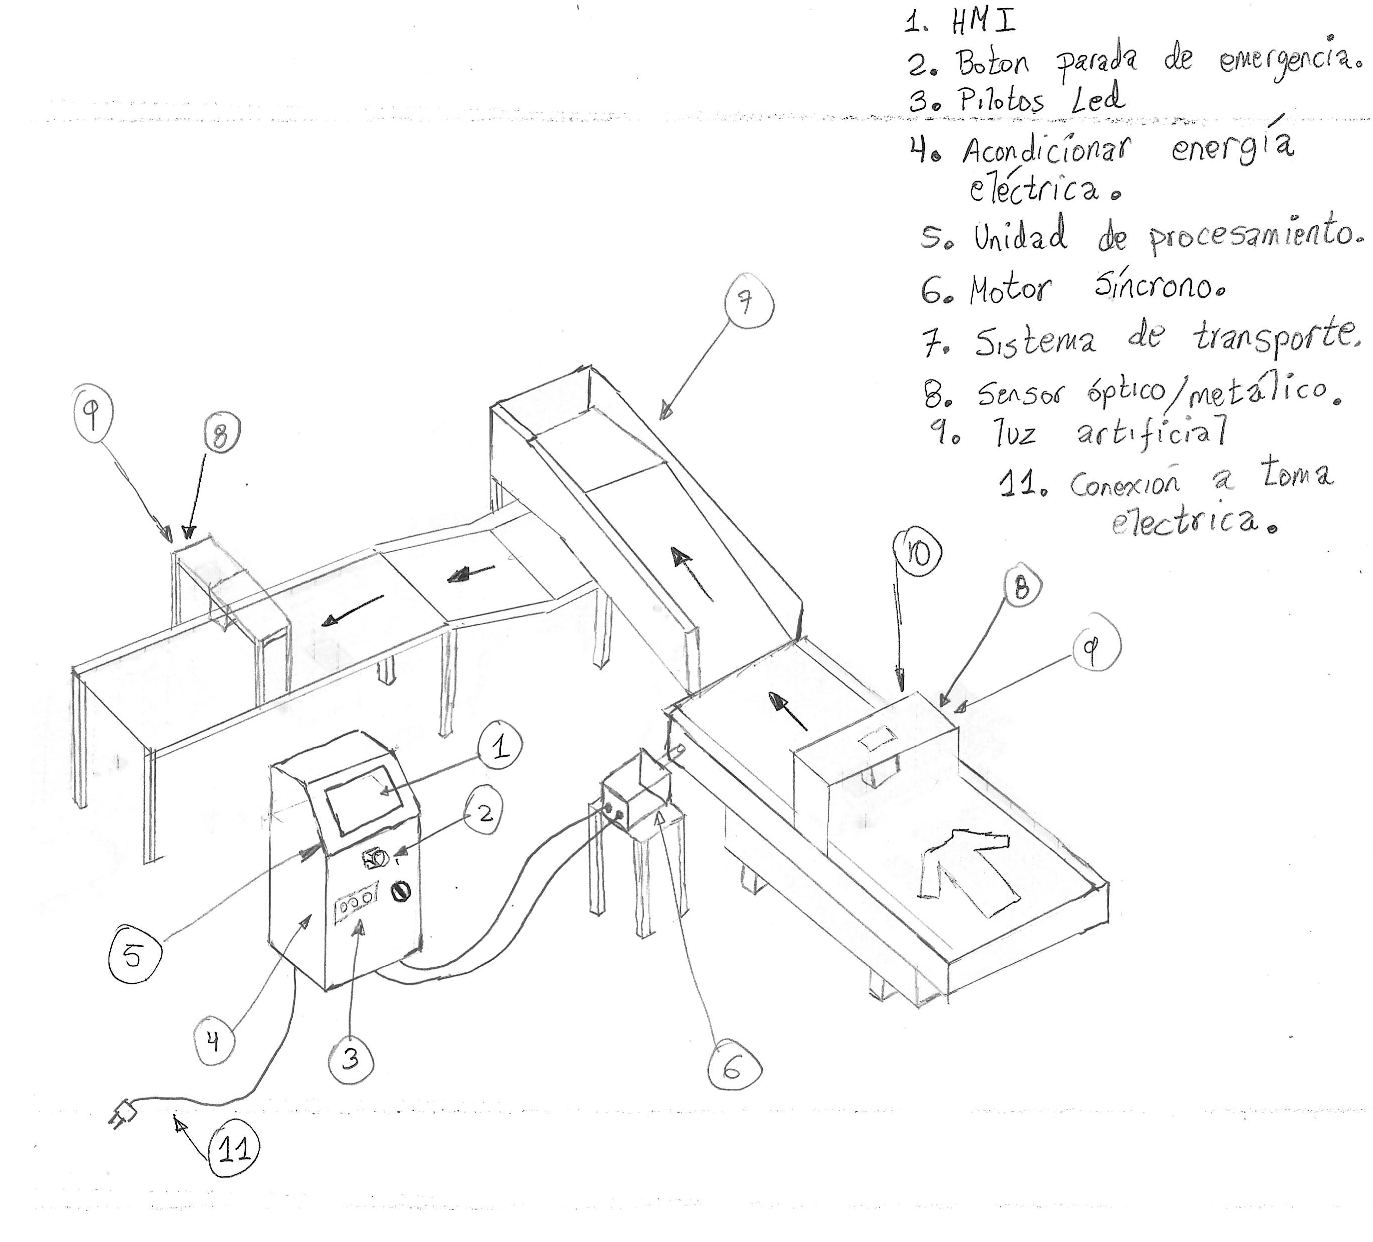
\includegraphics[page=1,width=\textwidth]{img/sketch_CS.pdf}
	\caption[Concepto solución 3.]{Concepto solución 3. Fuente: Elaboración propia.}
	\label{fig:sketch_CS_3}
\end{figure}

\section{Análisis técnico-económica}
% FELIX_RUIZ_JAVIER_DISEÑO_ELECTROGONIÓMETRO_MEDIR

Siguiendo la metodología VDI 2225 \cite{VDI2225_series}, se establecen criterios para evaluar los aspectos técnicos y económicos de las soluciones propuestas. La evaluación técnica y económica se presenta en las Tablas \ref{tab:eval_tecnica} y \ref{tab:eval_economica}, respectivamente. Los criterios tienen pesos diferenciados en el cálculo ponderado, reflejando su importancia en el sistema de acuerdo con la siguiente nomenclatura:

\begin{itemize}
\setlength\itemsep{0em}
	\item El valor de \textbf{g} representa el peso ponderado en función de la importancia del criterio de evaluación.
	\begin{itemize}
	\setlength\itemsep{0em}
		\item 1 = No importante.
		\item 2 = Poco importante.
		\item 3 = Importante.
		\item 4 = Muy importante.
	\end{itemize}
	\item El valor de \textbf{p} representa un puntaje de 0 a 4 (Escala de valores VDI 2225), siendo:
	\begin{itemize}
	\setlength\itemsep{0em}
		\item 0 = No satisface.
		\item 1 = Apenas aceptable.
		\item 2 = Suficiente.
		\item 3 = Bien.
		\item 4 = Excelente (Ideal).
	\end{itemize}
\end{itemize}
	

% Table generated by Excel2LaTeX from sheet 'EVALUACIONES'
\begin{table}[H]
	\centering
	\caption[Evaluación técnica de los conceptos de solución.]{Evaluación técnica de los conceptos de solución. Fuente: Elaboración propia.}
	\begin{tabular}{|c|c|c|c|c|c|c|c|c|c|c|}
		\hline
		\multicolumn{3}{|c|}{\textbf{Evaluación Técnica}} & \multicolumn{2}{c|}{\cellcolor[rgb]{ 1,  0,  0}\textcolor[rgb]{ 1,  1,  1}{\textbf{Solución 1}}} & \multicolumn{2}{c|}{\cellcolor[rgb]{ 0,  0,  1}\textcolor[rgb]{ 1,  1,  1}{\textbf{Solución 2}}} & \multicolumn{2}{c|}{\cellcolor[rgb]{ .298,  .835,  .078}\textbf{Solución 3}} & \multicolumn{2}{c|}{\cellcolor[rgb]{ 1,  .82,  .4}\textbf{Ideal}} \bigstrut\\
		\hline
		\textbf{Nro} & \textbf{Criterio} & \textbf{g} & \textbf{p} & \textbf{p x g} & \textbf{p} & \textbf{p x g} & \textbf{p} & \textbf{p x g} & \textbf{p} & \textbf{p x g} \bigstrut\\
		\hline
		\textbf{1} & \multicolumn{1}{l|}{\textbf{Tamaño}} & \multicolumn{1}{r|}{2} & \multicolumn{1}{r|}{\cellcolor[rgb]{ .949,  .863,  .859}3} & \multicolumn{1}{r|}{6} & \multicolumn{1}{r|}{\cellcolor[rgb]{ .863,  .902,  .945}3} & \multicolumn{1}{r|}{6} & \multicolumn{1}{r|}{\cellcolor[rgb]{ .922,  .945,  .871}2} & \multicolumn{1}{r|}{4} & \multicolumn{1}{r|}{\cellcolor[rgb]{ .992,  .914,  .851}4} & \multicolumn{1}{r|}{8} \bigstrut\\
		\hline
		\textbf{2} & \multicolumn{1}{l|}{\textbf{Dificultad de fabricación}} & \multicolumn{1}{r|}{2} & \multicolumn{1}{r|}{\cellcolor[rgb]{ .949,  .863,  .859}4} & \multicolumn{1}{r|}{8} & \multicolumn{1}{r|}{\cellcolor[rgb]{ .863,  .902,  .945}3} & \multicolumn{1}{r|}{6} & \multicolumn{1}{r|}{\cellcolor[rgb]{ .922,  .945,  .871}2} & \multicolumn{1}{r|}{4} & \multicolumn{1}{r|}{\cellcolor[rgb]{ .992,  .914,  .851}4} & \multicolumn{1}{r|}{8} \bigstrut\\
		\hline
		\textbf{3} & \multicolumn{1}{l|}{\textbf{Calibración}} & \multicolumn{1}{r|}{4} & \multicolumn{1}{r|}{\cellcolor[rgb]{ .949,  .863,  .859}1} & \multicolumn{1}{r|}{4} & \multicolumn{1}{r|}{\cellcolor[rgb]{ .863,  .902,  .945}4} & \multicolumn{1}{r|}{16} & \multicolumn{1}{r|}{\cellcolor[rgb]{ .922,  .945,  .871}2} & \multicolumn{1}{r|}{8} & \multicolumn{1}{r|}{\cellcolor[rgb]{ .992,  .914,  .851}4} & \multicolumn{1}{r|}{16} \bigstrut\\
		\hline
		\textbf{4} & \multicolumn{1}{l|}{\textbf{Tiempo de procesamiento}} & \multicolumn{1}{r|}{4} & \multicolumn{1}{r|}{\cellcolor[rgb]{ .949,  .863,  .859}2} & \multicolumn{1}{r|}{8} & \multicolumn{1}{r|}{\cellcolor[rgb]{ .863,  .902,  .945}4} & \multicolumn{1}{r|}{16} & \multicolumn{1}{r|}{\cellcolor[rgb]{ .922,  .945,  .871}4} & \multicolumn{1}{r|}{16} & \multicolumn{1}{r|}{\cellcolor[rgb]{ .992,  .914,  .851}4} & \multicolumn{1}{r|}{16} \bigstrut\\
		\hline
		\textbf{5} & \multicolumn{1}{l|}{\textbf{Interfaz intuitiva}} & \multicolumn{1}{r|}{3} & \multicolumn{1}{r|}{\cellcolor[rgb]{ .949,  .863,  .859}3} & \multicolumn{1}{r|}{9} & \multicolumn{1}{r|}{\cellcolor[rgb]{ .863,  .902,  .945}4} & \multicolumn{1}{r|}{12} & \multicolumn{1}{r|}{\cellcolor[rgb]{ .922,  .945,  .871}4} & \multicolumn{1}{r|}{12} & \multicolumn{1}{r|}{\cellcolor[rgb]{ .992,  .914,  .851}4} & \multicolumn{1}{r|}{12} \bigstrut\\
		\hline
		\textbf{6} & \multicolumn{1}{l|}{\textbf{Facilidad de manejo }} & \multicolumn{1}{r|}{4} & \multicolumn{1}{r|}{\cellcolor[rgb]{ .949,  .863,  .859}3} & \multicolumn{1}{r|}{12} & \multicolumn{1}{r|}{\cellcolor[rgb]{ .863,  .902,  .945}3} & \multicolumn{1}{r|}{12} & \multicolumn{1}{r|}{\cellcolor[rgb]{ .922,  .945,  .871}3} & \multicolumn{1}{r|}{12} & \multicolumn{1}{r|}{\cellcolor[rgb]{ .992,  .914,  .851}4} & \multicolumn{1}{r|}{16} \bigstrut\\
		\hline
		\textbf{7} & \multicolumn{1}{l|}{\textbf{Seguridad}} & \multicolumn{1}{r|}{4} & \multicolumn{1}{r|}{\cellcolor[rgb]{ .949,  .863,  .859}3} & \multicolumn{1}{r|}{12} & \multicolumn{1}{r|}{\cellcolor[rgb]{ .863,  .902,  .945}3} & \multicolumn{1}{r|}{12} & \multicolumn{1}{r|}{\cellcolor[rgb]{ .922,  .945,  .871}4} & \multicolumn{1}{r|}{16} & \multicolumn{1}{r|}{\cellcolor[rgb]{ .992,  .914,  .851}4} & \multicolumn{1}{r|}{16} \bigstrut\\
		\hline
		\textbf{8} & \multicolumn{1}{l|}{\textbf{Facilidad de mantenimiento}} & \multicolumn{1}{r|}{2} & \multicolumn{1}{r|}{\cellcolor[rgb]{ .949,  .863,  .859}3} & \multicolumn{1}{r|}{6} & \multicolumn{1}{r|}{\cellcolor[rgb]{ .863,  .902,  .945}2} & \multicolumn{1}{r|}{4} & \multicolumn{1}{r|}{\cellcolor[rgb]{ .922,  .945,  .871}3} & \multicolumn{1}{r|}{6} & \multicolumn{1}{r|}{\cellcolor[rgb]{ .992,  .914,  .851}4} & \multicolumn{1}{r|}{8} \bigstrut\\
		\hline
		\textbf{9} & \multicolumn{1}{l|}{\textbf{Durabilidad}} & \multicolumn{1}{r|}{2} & \multicolumn{1}{r|}{\cellcolor[rgb]{ .949,  .863,  .859}2} & \multicolumn{1}{r|}{4} & \multicolumn{1}{r|}{\cellcolor[rgb]{ .863,  .902,  .945}2} & \multicolumn{1}{r|}{4} & \multicolumn{1}{r|}{\cellcolor[rgb]{ .922,  .945,  .871}3} & \multicolumn{1}{r|}{6} & \multicolumn{1}{r|}{\cellcolor[rgb]{ .992,  .914,  .851}4} & \multicolumn{1}{r|}{8} \bigstrut\\
		\hline
		\rowcolor[rgb]{ .851,  .851,  .851} \multicolumn{3}{|c|}{\textbf{Suma}} & \multicolumn{1}{r|}{24} & \multicolumn{1}{r|}{69} & \multicolumn{1}{r|}{28} & \multicolumn{1}{r|}{88} & \multicolumn{1}{r|}{27} & \multicolumn{1}{r|}{84} & \multicolumn{1}{r|}{36} & \multicolumn{1}{r|}{108} \bigstrut\\
		\hline
		\multicolumn{3}{|c|}{\textbf{Promedio}} & \multicolumn{1}{r|}{0.667} & \multicolumn{1}{r|}{\cellcolor[rgb]{ 1,  1,  0}0.639} & \multicolumn{1}{r|}{0.778} & \multicolumn{1}{r|}{\cellcolor[rgb]{ 1,  1,  0}0.815} & \multicolumn{1}{r|}{0.750} & \multicolumn{1}{r|}{\cellcolor[rgb]{ 1,  1,  0}0.778} & \multicolumn{1}{r|}{1} & \multicolumn{1}{r|}{\cellcolor[rgb]{ 1,  1,  0}1} \bigstrut\\
		\hline
		\multicolumn{3}{|c|}{\textbf{Orden}} & \multicolumn{2}{c|}{3} & \multicolumn{2}{c|}{1} & \multicolumn{2}{c|}{2} & \multicolumn{2}{c|}{} \bigstrut\\
		\hline
	\end{tabular}%
	\label{tab:eval_tecnica}%
\end{table}%

% Table generated by Excel2LaTeX from sheet 'EVALUACIONES'
\begin{table}[H]
	\centering
	\caption[Evaluación económica de los conceptos de solución.]{Evaluación económica de los conceptos de solución. Fuente: Elaboración propia.}
	\begin{tabular}{|c|c|c|c|c|c|c|c|c|c|c|}
		\hline
		\multicolumn{3}{|c|}{\textbf{Evaluación Técnica}} & \multicolumn{2}{c|}{\cellcolor[rgb]{ 1,  0,  0}\textcolor[rgb]{ 1,  1,  1}{\textbf{Solución 1}}} & \multicolumn{2}{c|}{\cellcolor[rgb]{ 0,  0,  1}\textcolor[rgb]{ 1,  1,  1}{\textbf{Solución 2}}} & \multicolumn{2}{c|}{\cellcolor[rgb]{ .298,  .835,  .078}\textbf{Solución 3}} & \multicolumn{2}{c|}{\cellcolor[rgb]{ 1,  .82,  .4}\textbf{Ideal}} \bigstrut\\
		\hline
		\textbf{Nro} & \textbf{Criterio} & \textbf{g} & \textbf{p} & \textbf{p x g} & \textbf{p} & \textbf{p x g} & \textbf{p} & \textbf{p x g} & \textbf{p} & \textbf{p x g} \bigstrut\\
		\hline
		\textbf{1} & \multicolumn{1}{l|}{\textbf{Número de piezas}} & \multicolumn{1}{r|}{2} & \multicolumn{1}{r|}{\cellcolor[rgb]{ .949,  .863,  .859}3} & \multicolumn{1}{r|}{6} & \multicolumn{1}{r|}{\cellcolor[rgb]{ .863,  .902,  .945}3} & \multicolumn{1}{r|}{6} & \multicolumn{1}{r|}{\cellcolor[rgb]{ .922,  .945,  .871}3} & \multicolumn{1}{r|}{6} & \multicolumn{1}{r|}{\cellcolor[rgb]{ .992,  .914,  .851}4} & \multicolumn{1}{r|}{8} \bigstrut\\
		\hline
		\textbf{2} & \multicolumn{1}{l|}{\textbf{Costo de componentes}} & \multicolumn{1}{r|}{3} & \multicolumn{1}{r|}{\cellcolor[rgb]{ .949,  .863,  .859}3} & \multicolumn{1}{r|}{9} & \multicolumn{1}{r|}{\cellcolor[rgb]{ .863,  .902,  .945}3} & \multicolumn{1}{r|}{9} & \multicolumn{1}{r|}{\cellcolor[rgb]{ .922,  .945,  .871}2} & \multicolumn{1}{r|}{6} & \multicolumn{1}{r|}{\cellcolor[rgb]{ .992,  .914,  .851}4} & \multicolumn{1}{r|}{12} \bigstrut\\
		\hline
		\textbf{3} & \multicolumn{1}{l|}{\textbf{Disponibilidad de materiales}} & \multicolumn{1}{r|}{4} & \multicolumn{1}{r|}{\cellcolor[rgb]{ .949,  .863,  .859}3} & \multicolumn{1}{r|}{12} & \multicolumn{1}{r|}{\cellcolor[rgb]{ .863,  .902,  .945}2} & \multicolumn{1}{r|}{8} & \multicolumn{1}{r|}{\cellcolor[rgb]{ .922,  .945,  .871}1} & \multicolumn{1}{r|}{4} & \multicolumn{1}{r|}{\cellcolor[rgb]{ .992,  .914,  .851}4} & \multicolumn{1}{r|}{16} \bigstrut\\
		\hline
		\textbf{4} & \multicolumn{1}{l|}{\textbf{Costo de Tecnología}} & \multicolumn{1}{r|}{4} & \multicolumn{1}{r|}{\cellcolor[rgb]{ .949,  .863,  .859}2} & \multicolumn{1}{r|}{8} & \multicolumn{1}{r|}{\cellcolor[rgb]{ .863,  .902,  .945}3} & \multicolumn{1}{r|}{12} & \multicolumn{1}{r|}{\cellcolor[rgb]{ .922,  .945,  .871}2} & \multicolumn{1}{r|}{8} & \multicolumn{1}{r|}{\cellcolor[rgb]{ .992,  .914,  .851}2} & \multicolumn{1}{r|}{8} \bigstrut\\
		\hline
		\textbf{5} & \multicolumn{1}{l|}{\textbf{Costo de Fabricación}} & \multicolumn{1}{r|}{4} & \multicolumn{1}{r|}{\cellcolor[rgb]{ .949,  .863,  .859}3} & \multicolumn{1}{r|}{12} & \multicolumn{1}{r|}{\cellcolor[rgb]{ .863,  .902,  .945}4} & \multicolumn{1}{r|}{16} & \multicolumn{1}{r|}{\cellcolor[rgb]{ .922,  .945,  .871}2} & \multicolumn{1}{r|}{8} & \multicolumn{1}{r|}{\cellcolor[rgb]{ .992,  .914,  .851}4} & \multicolumn{1}{r|}{16} \bigstrut\\
		\hline
		\textbf{6} & \multicolumn{1}{l|}{\textbf{Costo de Mantenimiento}} & \multicolumn{1}{r|}{2} & \multicolumn{1}{r|}{\cellcolor[rgb]{ .949,  .863,  .859}2} & \multicolumn{1}{r|}{4} & \multicolumn{1}{r|}{\cellcolor[rgb]{ .863,  .902,  .945}2} & \multicolumn{1}{r|}{4} & \multicolumn{1}{r|}{\cellcolor[rgb]{ .922,  .945,  .871}2} & \multicolumn{1}{r|}{4} & \multicolumn{1}{r|}{\cellcolor[rgb]{ .992,  .914,  .851}4} & \multicolumn{1}{r|}{8} \bigstrut\\
		\hline
		\rowcolor[rgb]{ .851,  .851,  .851} \multicolumn{3}{|c|}{\textbf{Suma}} & \multicolumn{1}{r|}{16} & \multicolumn{1}{r|}{51} & \multicolumn{1}{r|}{17} & \multicolumn{1}{r|}{55} & \multicolumn{1}{r|}{12} & \multicolumn{1}{r|}{36} & \multicolumn{1}{r|}{22} & \multicolumn{1}{r|}{68} \bigstrut\\
		\hline
		\multicolumn{3}{|c|}{\textbf{Promedio}} & \multicolumn{1}{r|}{0.727} & \multicolumn{1}{r|}{\cellcolor[rgb]{ 1,  1,  0}0.750} & \multicolumn{1}{r|}{0.773} & \multicolumn{1}{r|}{\cellcolor[rgb]{ 1,  1,  0}0.809} & \multicolumn{1}{r|}{0.545} & \multicolumn{1}{r|}{\cellcolor[rgb]{ 1,  1,  0}0.529} & \multicolumn{1}{r|}{1} & \multicolumn{1}{r|}{\cellcolor[rgb]{ 1,  1,  0}1} \bigstrut\\
		\hline
		\multicolumn{3}{|c|}{\textbf{Orden}} & \multicolumn{2}{c|}{2} & \multicolumn{2}{c|}{1} & \multicolumn{2}{c|}{3} & \multicolumn{2}{c|}{} \bigstrut\\
		\hline
	\end{tabular}%
	\label{tab:eval_economica}%
\end{table}%


Basándonos en los datos de las Tablas \ref{tab:eval_tecnica} y \ref{tab:eval_economica}, realizamos un estudio técnico y económico que nos permite identificar la mejor solución. La Figura \ref{fig:comp_tecnico_economica} muestra un gráfico comparativo de las tres soluciones sugeridas frente a una línea que simboliza el equilibrio ideal.

\begin{figure}[H]
	\centering
	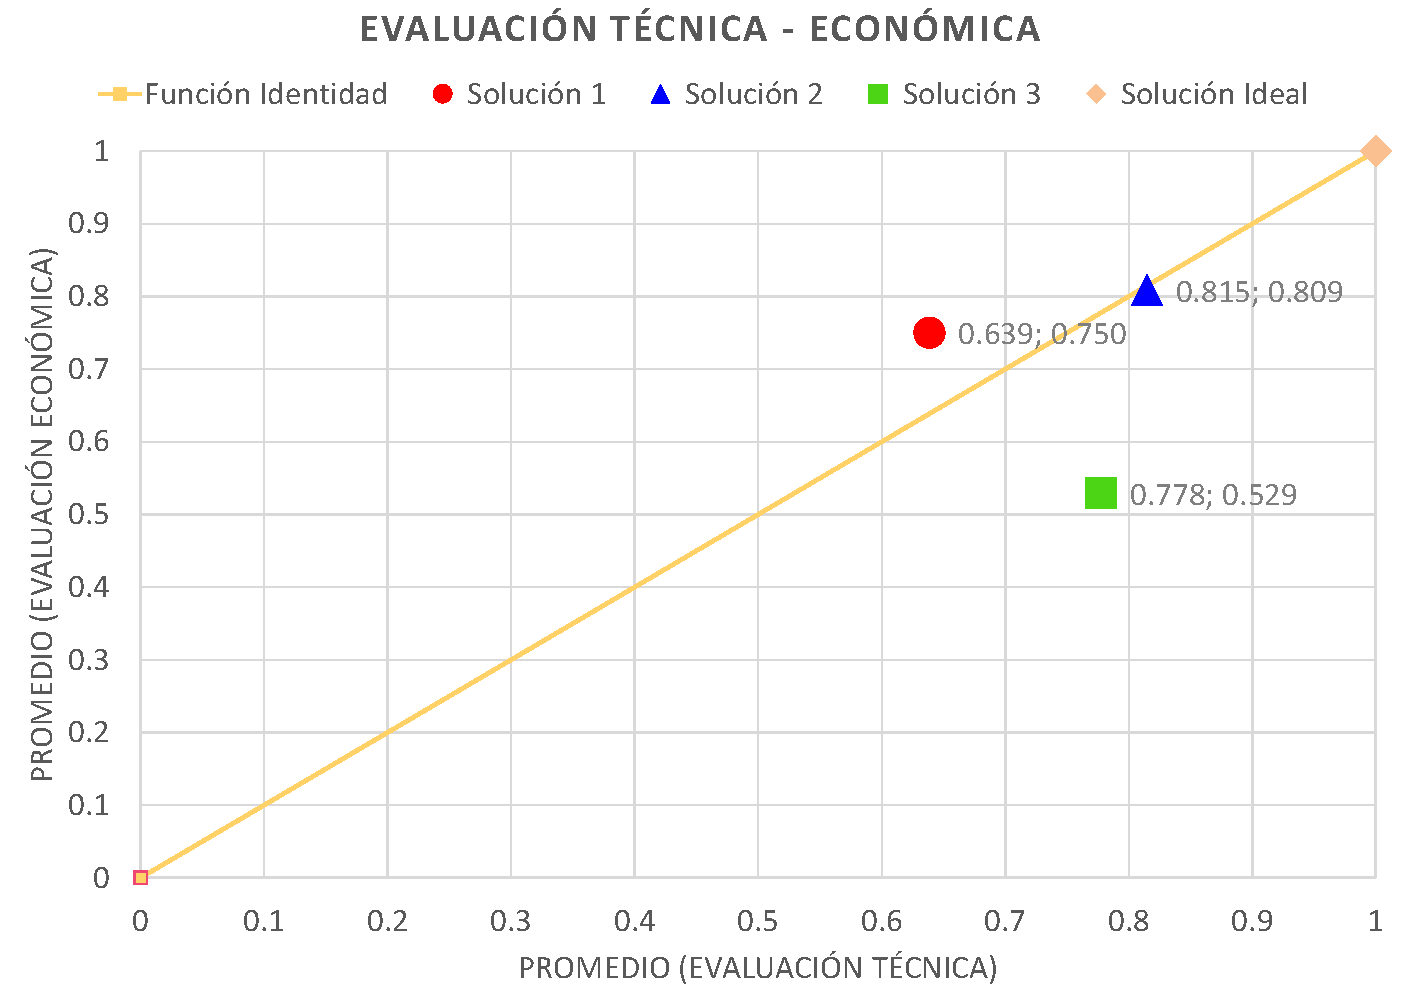
\includegraphics[width=0.9\textwidth]{img/comp_tecnico_economica.pdf}
	\caption[Gráfica de comparación técnico-económica de los conceptos de solución.]{Gráfica de comparación técnico-económica de los conceptos de solución. Fuente: Elaboración propia.}
	\label{fig:comp_tecnico_economica}
\end{figure}

Se observa que la solución que esta más cerca de la solución ideal es la \textbf{Solución 2}, en comparación con las otras opciones. Esta solución también demuestra un balance adecuado entre los aspectos económicos y técnicos, ya que se encuentra próxima a la línea de equilibrio ideal. Por lo tanto, elegimos esta solución como punto de partida para el diseño ingenieril, el cual será explorado en detalle en los siguientes capítulos.
